\section{Analysis of hidden activation vectors}
\label{sec:macro}

\begin{figure*}[t]
\hspace*{-0.5in}
\setlength{\tabcolsep}{0.01pt}
    \begin{tabular}{cccc}
    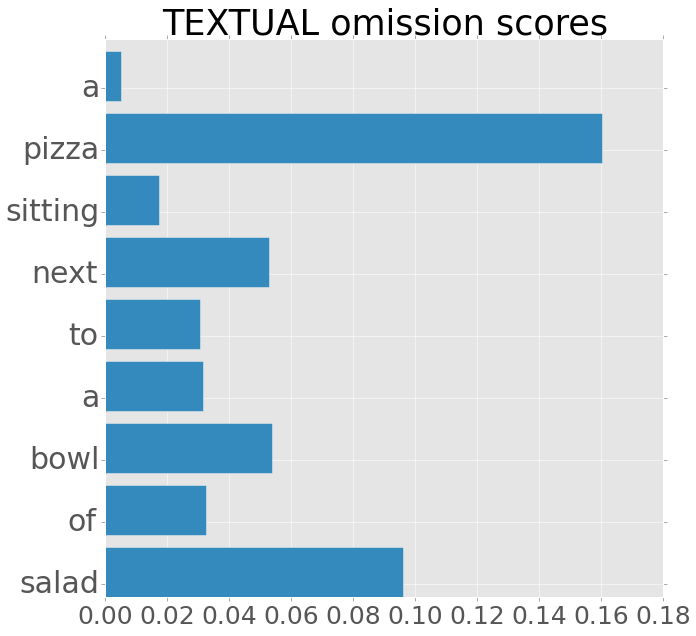
\includegraphics[scale=0.14]{new_omission_examples/textual1} &
    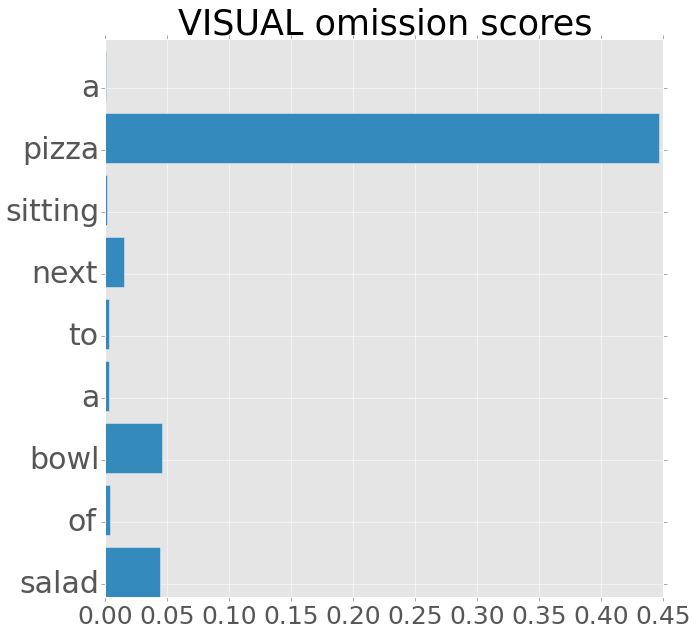
\includegraphics[scale=0.14]{new_omission_examples/visual1} &
    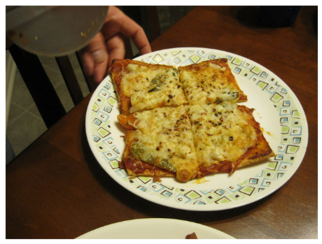
\includegraphics[scale=0.33]{new_omission_examples/img1} & 
    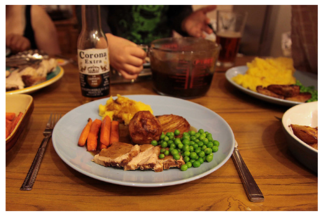
\includegraphics[scale=0.28]{new_omission_examples/img1_omit} \\
    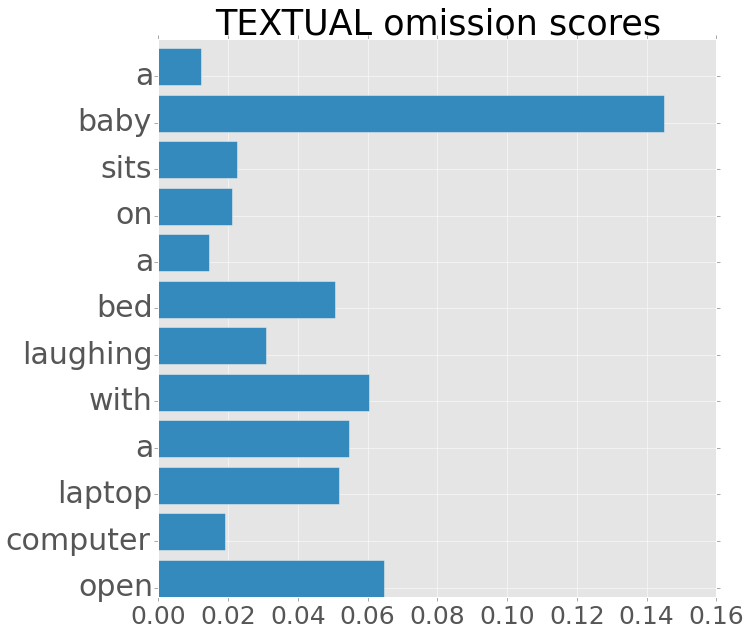
\includegraphics[scale=0.16]{new_omission_examples/textual2} &
    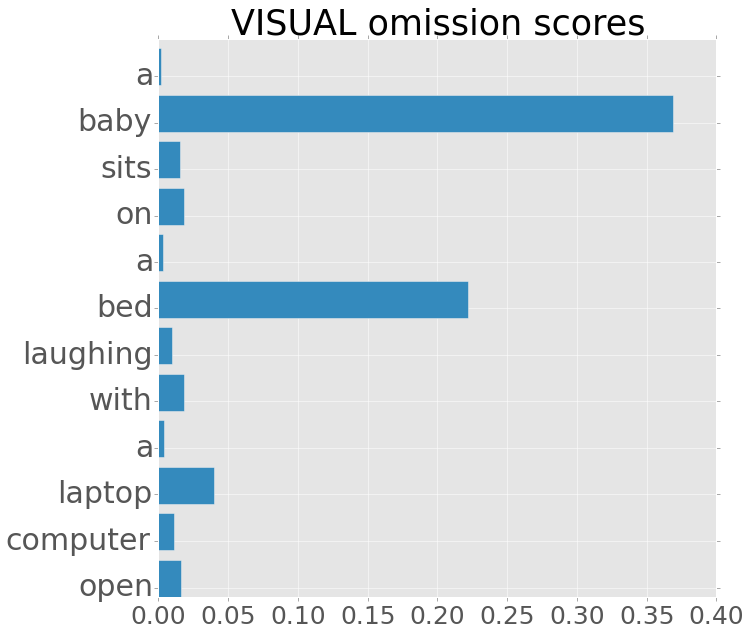
\includegraphics[scale=0.16]{new_omission_examples/visual2} &
    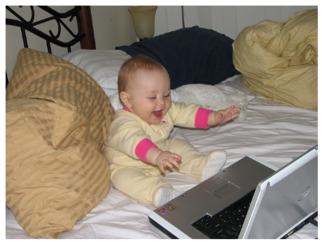
\includegraphics[scale=0.28]{new_omission_examples/img2} & 
    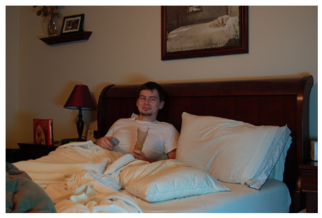
\includegraphics[scale=0.30]{new_omission_examples/img2_omit}
    \end{tabular}
    \caption{The omission scores of {\sc Visual} and {\sc Textual} for two example sentences, 
and the best retrieved images for the original sentence (left) and the sentence with the most 
important word removed (right). 
%Top row example caption is {\it a bottle next to a windowsill with
%  light coming through},  bottom row: {\it a train on a track next to
%  many bushes}.
}
    \label{fig:omissionex}
\end{figure*}

%Understanding the behavior of the learned models in terms of which features do they assign 
%the most attention to is straight forward with linear 
%models such as linear/logistic regression, 
%naive-bayes classifiers or with some of the non-parametric models as well such as decision 
%trees. This information allows researchers to not only train learning algorithms to perform 
%particular tasks, but also to uncover some underlying patterns in the training data. 
 
%\subsection{Salience of categories of words}
%\label{sec:salience}
In this section we propose novel techniques for interpreting the
activation patterns of neural networks trained on language tasks
from a linguistic point of view and focus
on the high level understanding of what types of words the networks
pay most attention to. Furthermore, we investigate if the networks
learn to assign appropriate amounts of importance to tokens depending
on their position and grammatical function in the sentences.\label{edit:whyposdep}
In Section \ref{sec:computeomission} we introduce \emph{omission scores};
a metric to measure the contribution of each token to the prediction of the networks.
Section \ref{sec:omitimaginet} aggregates the omission scores in terms
of dependency relations and part-of-speech categories and compares {\sc Visual}
and {\sc Textual}. Lastly Section \ref{sec:beyondlexical} investigates the extent to which
the importance of words for the different pathways depend on the words themselves,
their position and their grammatical function in the sentences.
% MAYBE THIS WOULD BE TOO MUCH
%We apply the proposed methods to explore
%the representations of {\sc Imaginet}, but also discuss how to generalize
%them to other architectures.

\subsection{Computing Omission Scores}
\label{sec:computeomission}

In both pathways of {\sc Imaginet} the full sentences are represented by the
activation vector at the end-of-sentence symbol
($\mathbf{h}_\text{end}$). We measure the salience of each word $S_i$
in an input sentence $S_{1:n}$ based on how much the representation of the
partial sentence $S_{\setminus i} = S_{1:i-1}S_{i+1:n}$, with
the omitted word $S_i$, deviates from that of the original sentence
representation. For example, the distance
between $\mathbf{h}_\text{end}(${\it the black dog is running}$)$
and $\mathbf{h}_\text{end}(${\it the dog is running}$)$ determines
the importance of {\it black} in the first sentence. We introduce the
measure $\mathrm{omission}(i,S)$ for estimating the salience of a word $S_i$:

\begin{equation}
\label{eg:omit}
\mathrm{omission}(i,S) = 1-\mathrm{cosine}(\mathbf{h}_\text{end}(S),
\mathbf{h}_\text{end}(S_{\setminus i}))
\end{equation}

\noindent Figure~\ref{fig:omissionex} demonstrates the omission
measure for the {\sc Visual} and {\sc Textual} pathways for two
example captions. For both captions the $\mathrm{omission}$ scores are
plotted along with the first image retrieved by {\sc Visual} for the
full sentence and for the sentence with the word with the highest
$\mathrm{omission}(i,S)$ removed. The images are retrieved from the
validation set of MS-COCO by: 1) computing the image representation of the 
given sentence with {\sc Visual}; 2) extracting the CNN features for the 
images from the set; and 3) finding the image that minimizes the cosine distance
to the query.\label{edit:retrievalexplain} 
In the first example, the omission
scores for {\sc Visual} suggest that the model interpreted {\it  pizza} as the most important
word in the sequence and returned an image that depicts a pizza on a plate. 
Removing the word {\it pizza} promotes {\it salad} and {\it bowl} as
the main theme of the sentence and the model retrieves an image with a dining table 
with salad-like dishes. 
For the second example, the omission scores for {\sc
  Visual} show that the model paid attention mostly to {\it baby} and
{\it bed} and slightly to {\it laptop} and retrieved an image depicting a baby 
sitting on a bed with a laptop.
Removing the word {\it baby} leads
to an image that depicts an adult male laying on a bed. Figure~\ref{fig:omissionex}
also shows that in contrast to {\sc Visual}, in both examples {\sc
  Textual} distributes its attention more evenly across time steps
instead of focusing on the types of words related to the corresponding
visual scene.


For other RNN architectures such as GRUs, LSTMs \label{edit:omitgeneral}
and their bi-directional variants, measuring the contribution
of tokens to their predictions the $\mathrm{omission}$ 
can be straight-forwardly computed using their hidden state 
at the last time step used for prediction. Furthermore, the technique 
can be applied in general to other architectures which
embed variable length linguistic expressions to the same fixed dimensional
space and perform predictions based on these embeddings. 
This includes tree-structured Recursive Neural Network models such as the Tree-LSTM
introduced in \namecite{kai2015treelstm} or the CNN architecture of \namecite{yoonneural2014} 
for sentence classification. In both cases the pre-softmax activations can be extracted 
from the models as the representations of the full and partial sentences.   


% Given a corpus segmented into sentences, each word in an input sentence is tagged with its 
%part-of-speech category (POS) and dependency-relation (DepRel). For dependency relations 
%only the label of the ark (and not the ark itself) is taken into account. For each input sentence 
%of 
%length $n$ the RNNs produce $n$ hidden activation vectors $h_{1}, \ldots , h_{n}$. Each word 
%in the input sentence is tagged with POS and DepRel categories and the contribution of the $<
%$word, POS, DepRel$>$ tuples to the meaning of the sentence is measured by computing the 
%following scores:
% 

%\paragraph{$omission$} Given a sentence "the black dog", we generate 3 sentence by 
%omitting one of the words each time: "the black", "the dog", "black dog". For each of these 
%sentence we compute a sentence representation $h_{full}$ and calculate the cosine 
%similarities 
%between the original and the omitted sentences. This measured is used to indicate the overall 
%importance of word categories. \todo{Example with a short sentence: ab, bc, cd, cosines}
%\\

%-----------------
\subsection{Omission score distributions}
\label{sec:omitimaginet}

%\begin{figure*}
 %   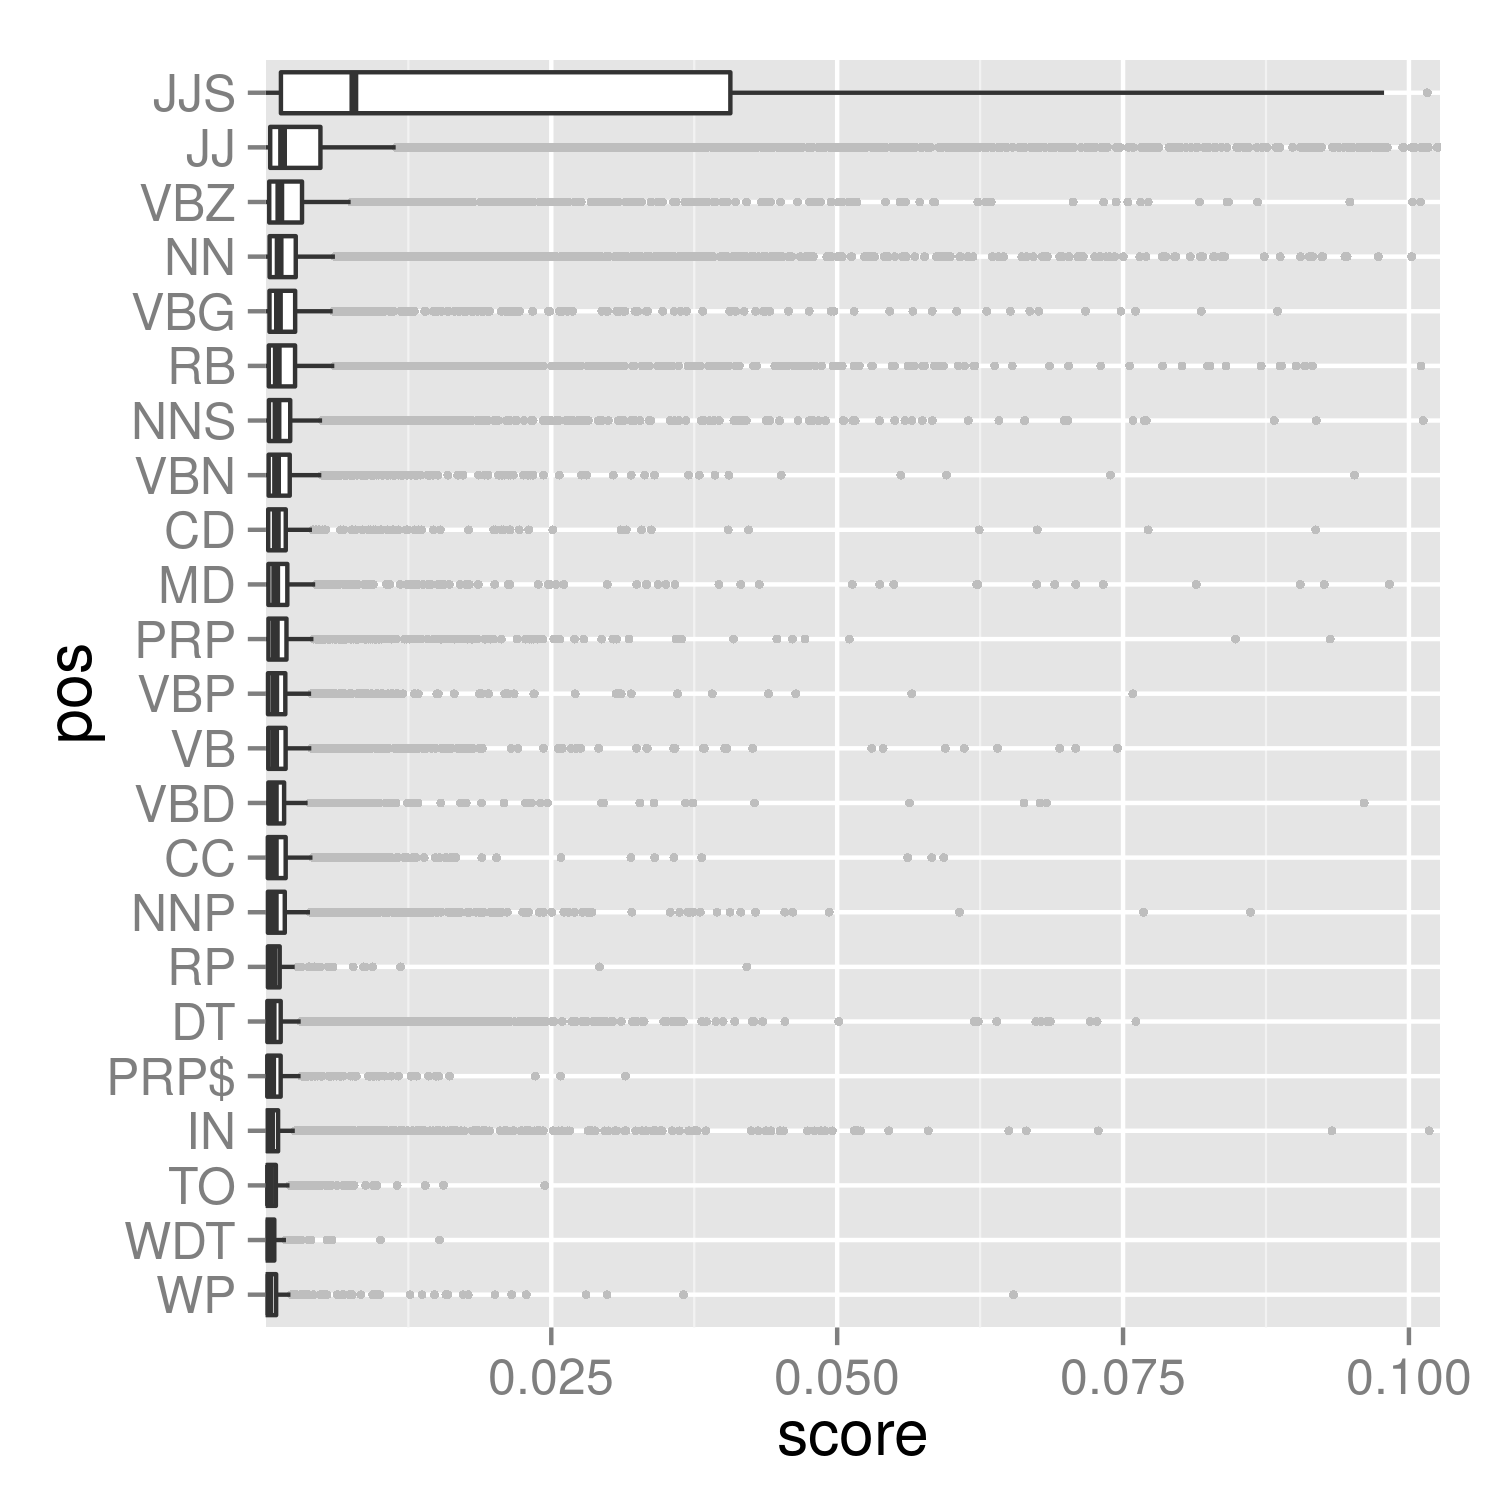
\includegraphics[scale=0.6]{omission-stat/sent-omission-pos-boxplot.png} 
 %   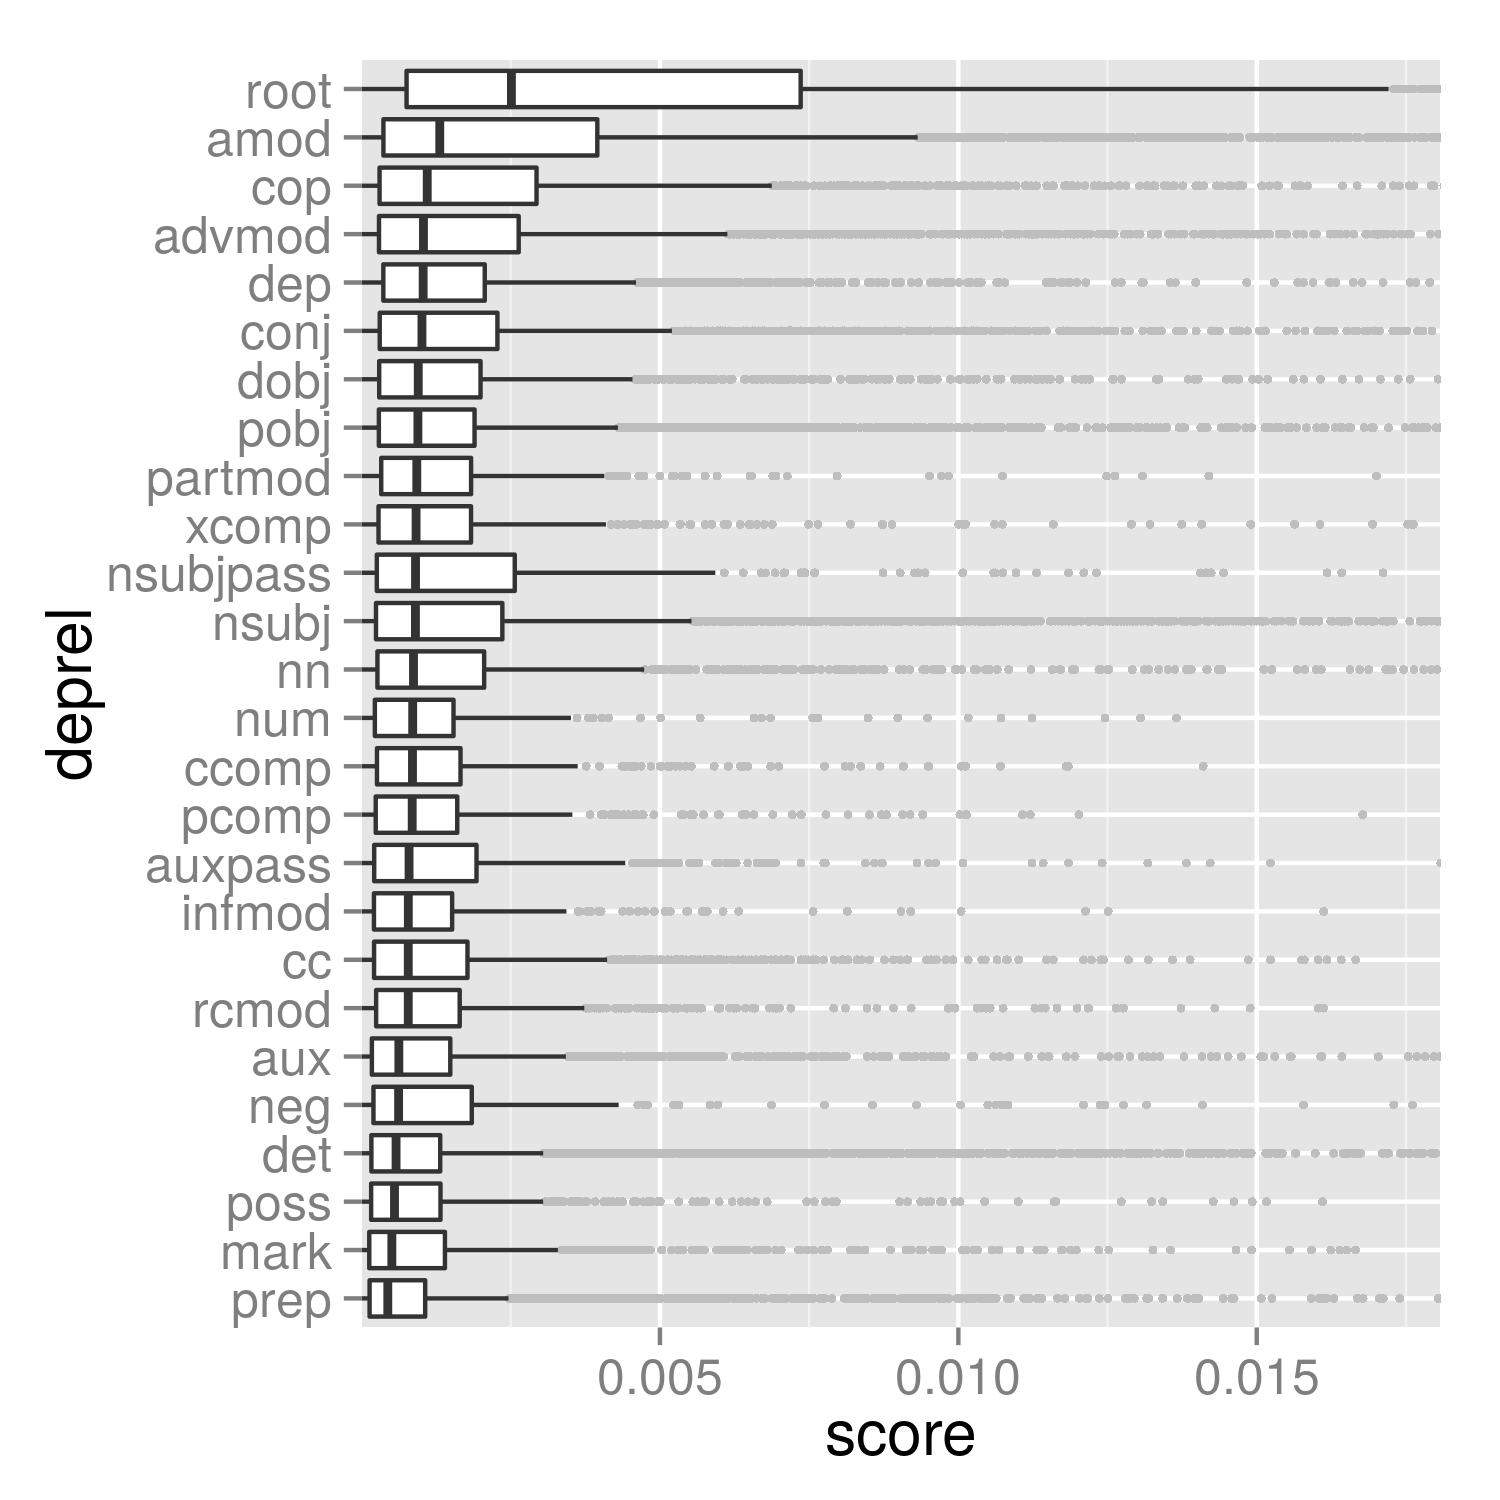
\includegraphics[scale=0.6]{omission-stat/sent-omission-deprel-boxplot.png} 
 %   \caption{Distributions of omission scores per POS category (left)
 %     and dependency relation (right) for {\sc Sentiment}. Only labels
 %   which occurred at least 300 times are included.}
%\label{fig:omission-sent}
%\end{figure*}

%\subsubsection{Omission results for {\sc Sentiment}}
%\label{sec:omitsentiment}
%Figure~\ref{fig:omission-sent} shows the distribution of the omission scores per category for the {\sc Sentiment} model. Superlative adjectives (JJS) such as {\it best, least, scaries} and {\it funniest} are by far the most influential POS category, followed by Adjectives (JJ), Verbs (VBZ, VBG), Nouns (NN, NNS) and Adverbs (RB). Similarly, tokens with function {\sc root} (various verbs, nouns or adjectives central to the meaning of the sentence) are recognized by the model as the most important category, followed by adjectival modifier {\sc amod}. These results support the validity of $\mathrm{omission}$ as a measure of saliency and provide evidence that {\sc Sentiment} learns representations that enable the model to successfully filter out irrelevant parts of the input. 

%-----------------
\label{subsec:omission-text-vis}
\begin{figure*}[t]
%\hspace*{-0.3in}
\setlength{\tabcolsep}{0pt}
  \begin{tabular}{cc}
  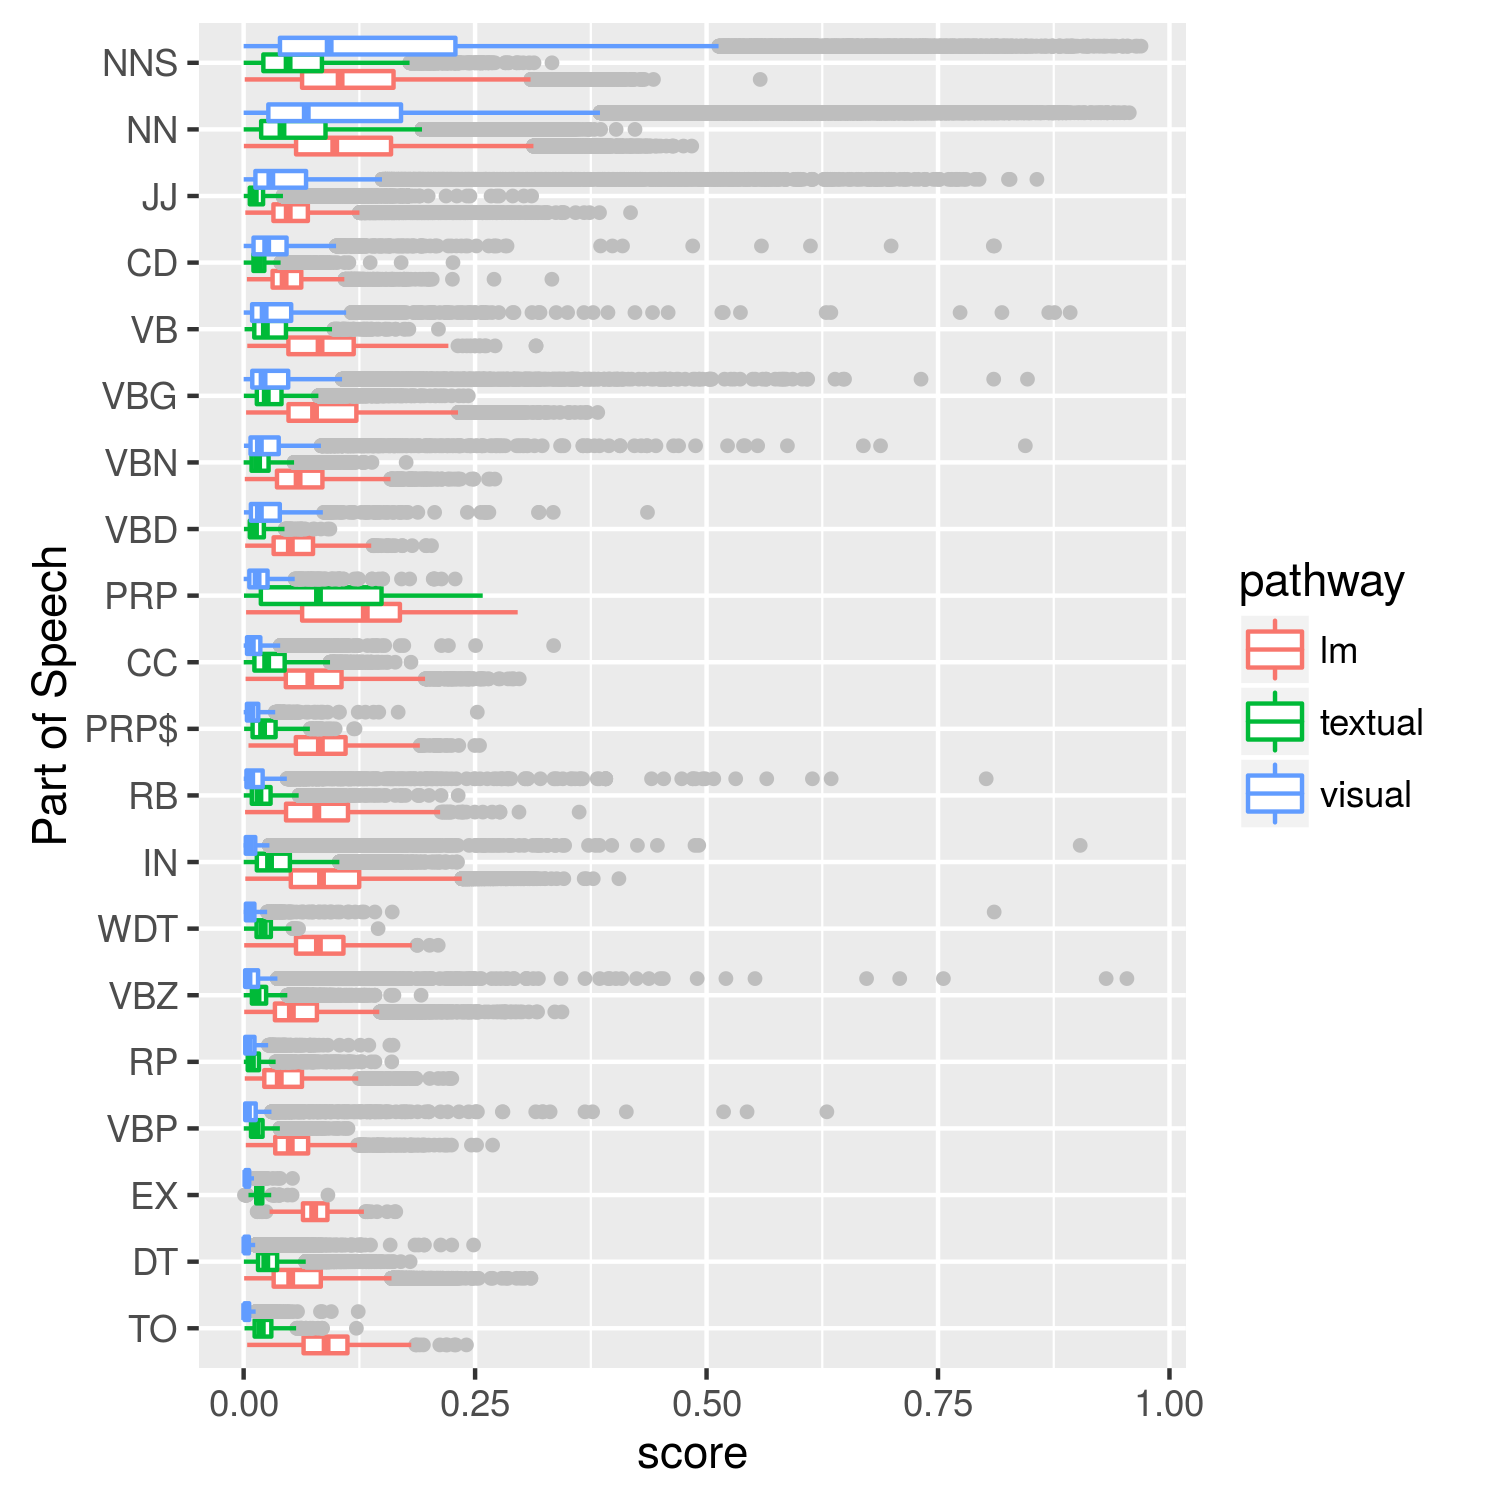
\includegraphics[scale=0.6]{imaginet-omission-pos-boxplot.png} &
  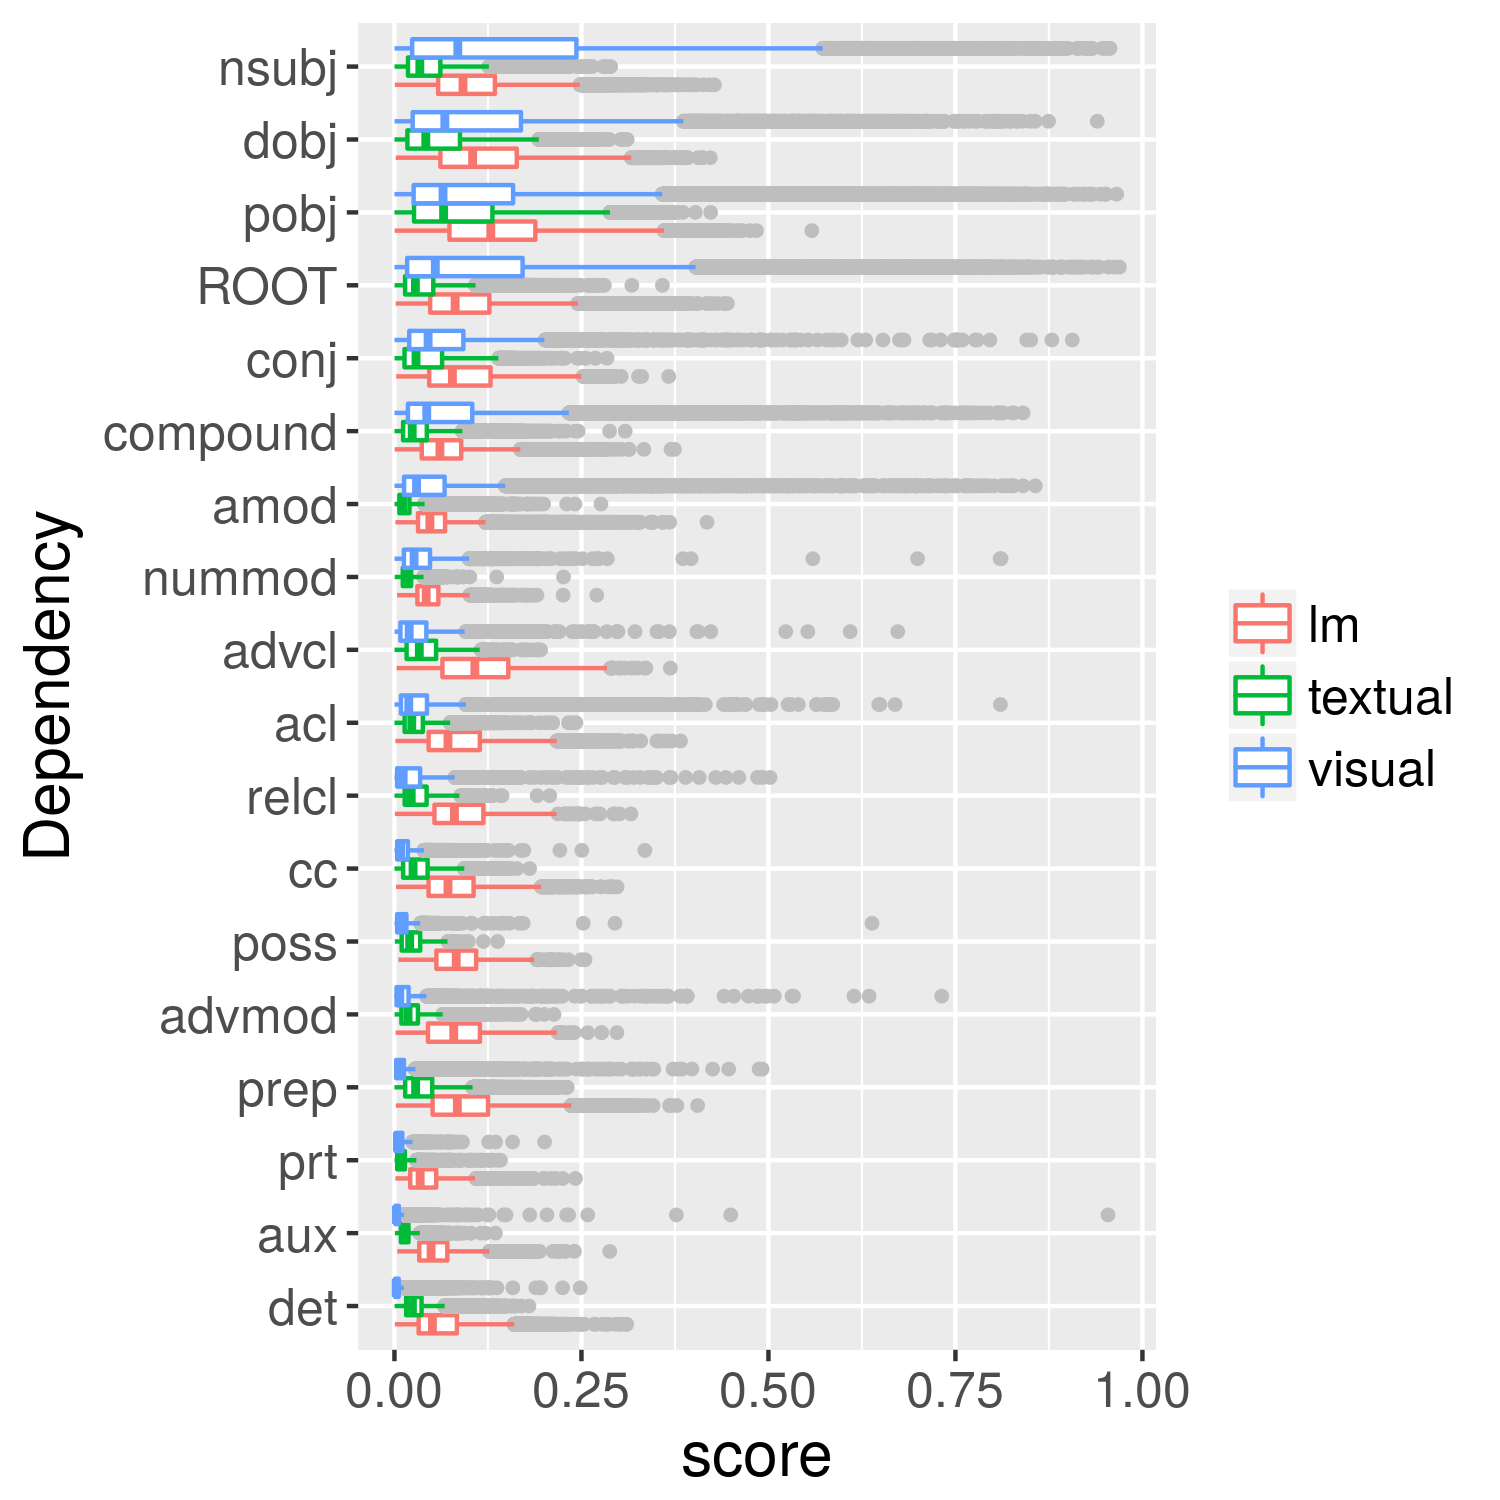
\includegraphics[scale=0.6]{imaginet-omission-dep-boxplot.png} \\
  \end{tabular}
  
\caption{Distribution of omission scores for POS (left) and dependency labels
  (right), for the {\sc Textual} and {\sc Visual} pathways. Only labels which occur at least 500 times are included.}
\label{fig:omission-imaginet}
\end{figure*}

\begin{figure*}[t]
  \centering
  \hspace*{-0.2in}
  \setlength{\tabcolsep}{0pt}
  \begin{tabular}{cc}
  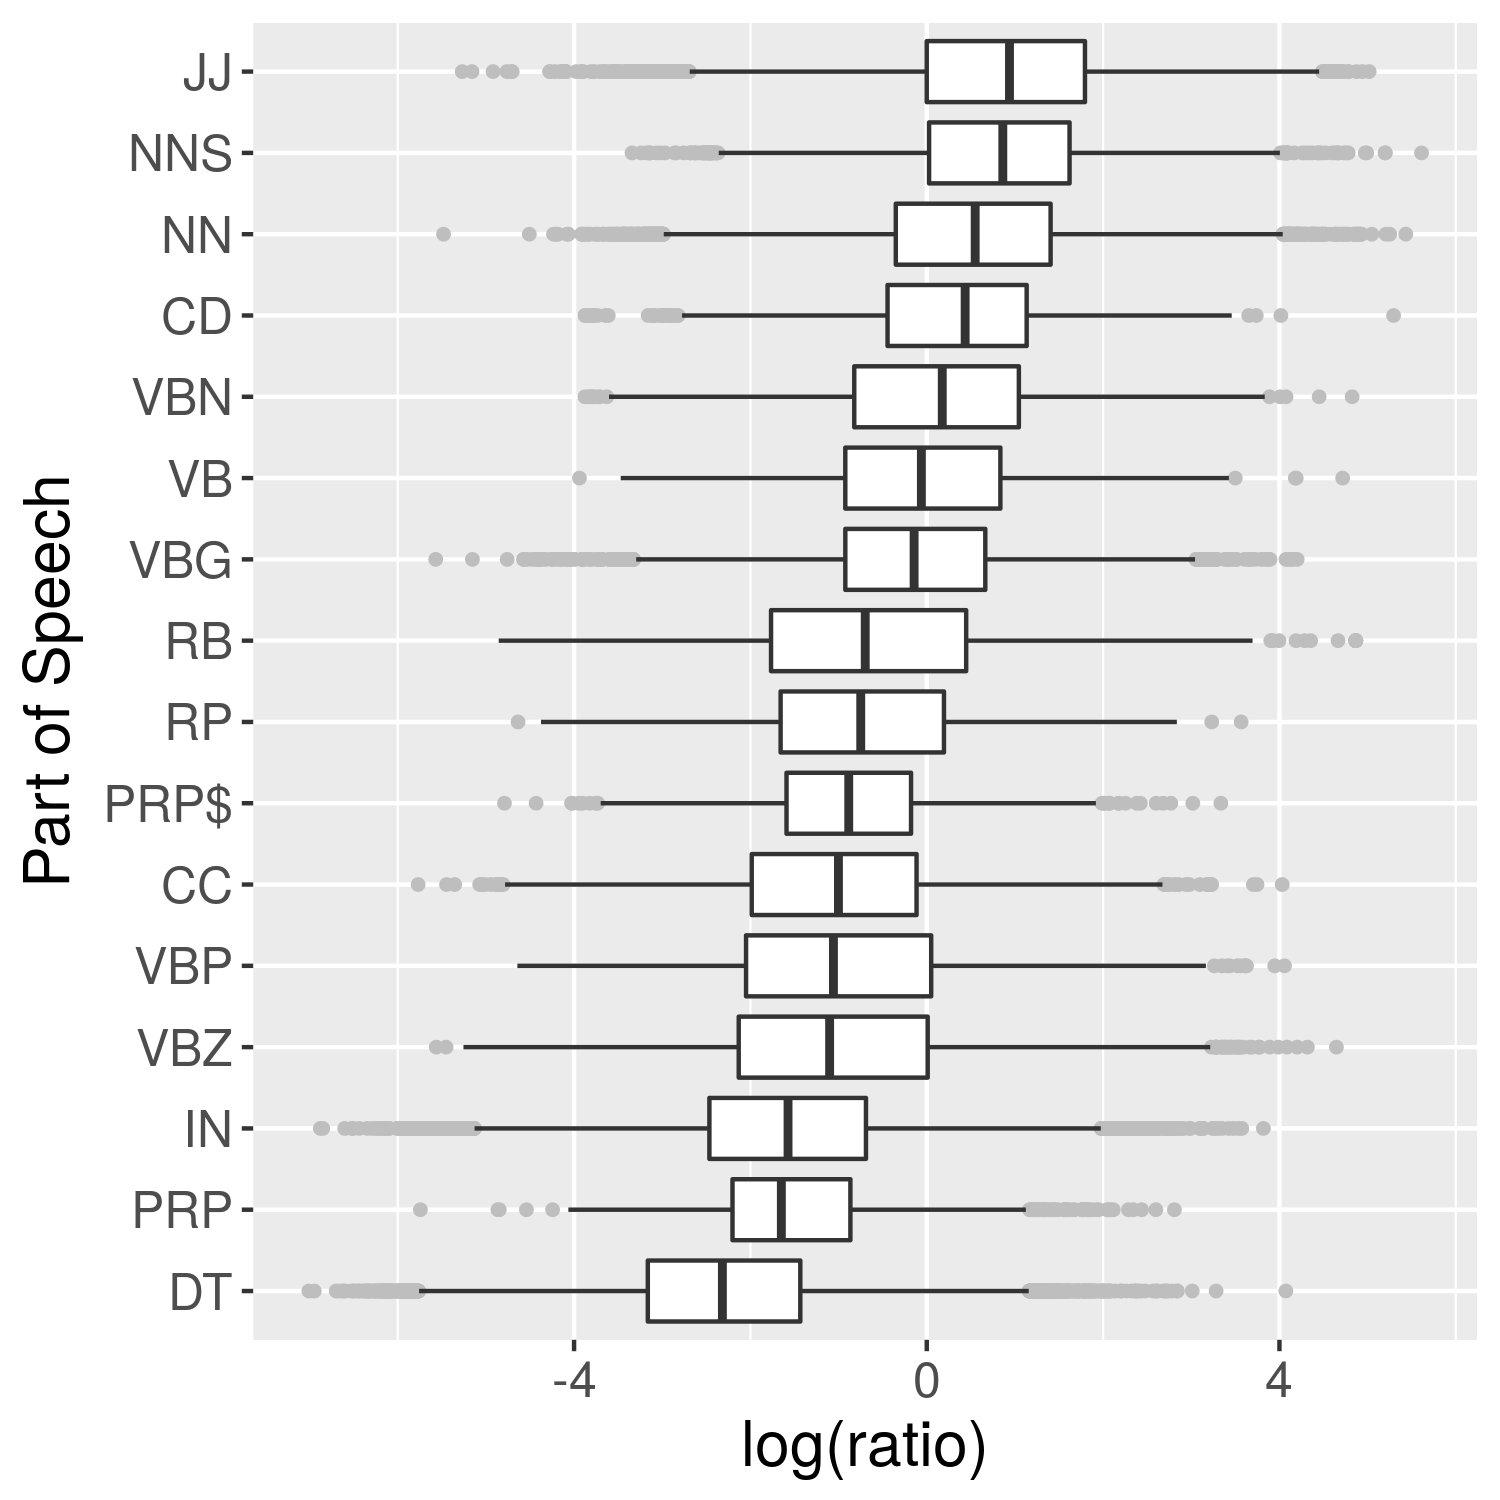
\includegraphics[scale=0.55]{imaginet-omission-ratio-pos-boxplot.png} &
  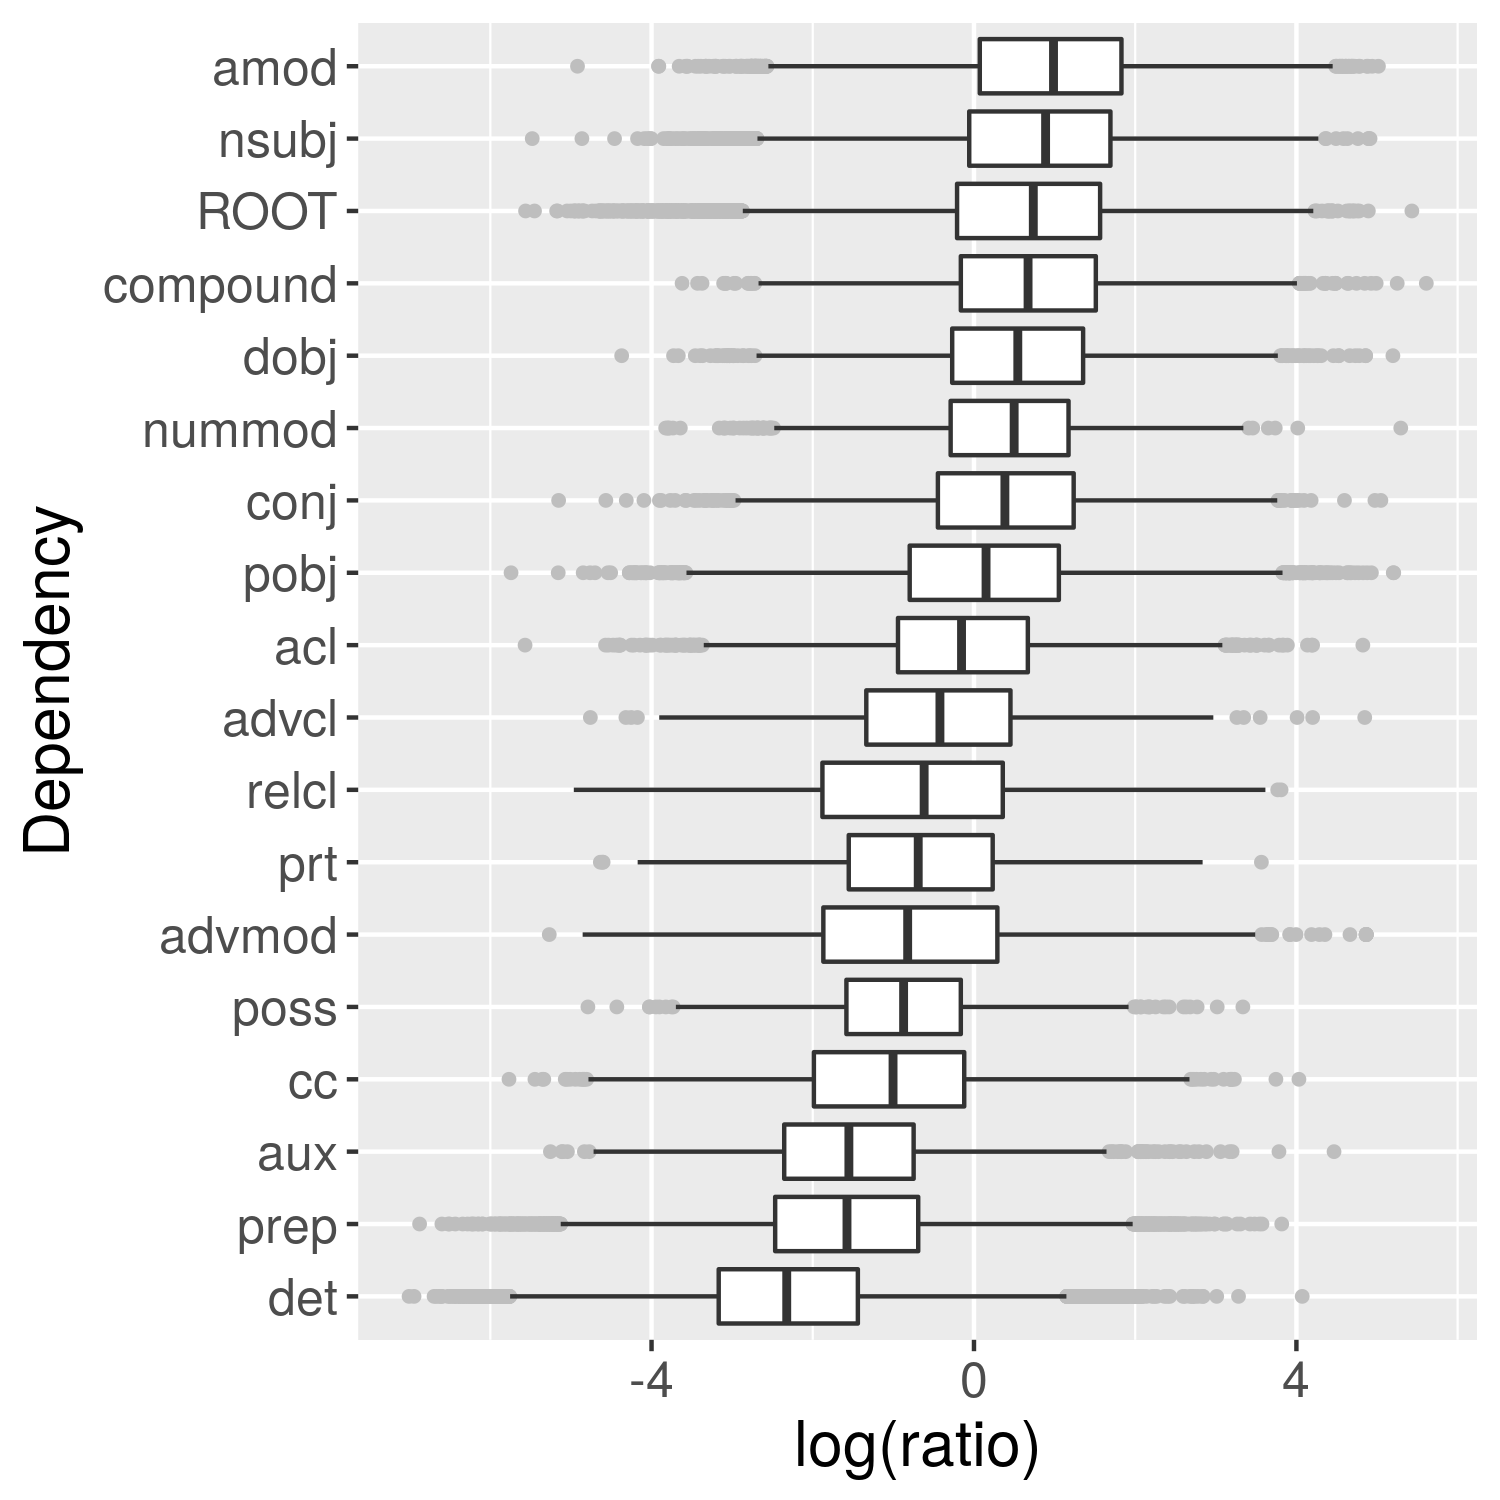
\includegraphics[scale=0.55]{imaginet-omission-ratio-dep-boxplot.png} \\  
  \end{tabular}
  \caption{Distributions of log ratios of omission scores of {\sc Textual} to {\sc Visual} per
    POS (left) and dependency labels (right). Only labels which occur at least 500 times are included.}
\label{fig:omission-imaginet-ratio}
\end{figure*}

\begin{figure*}[t]
  \centering
  \hspace*{-0.2in}
  \setlength{\tabcolsep}{0pt}
  \begin{tabular}{cc}
  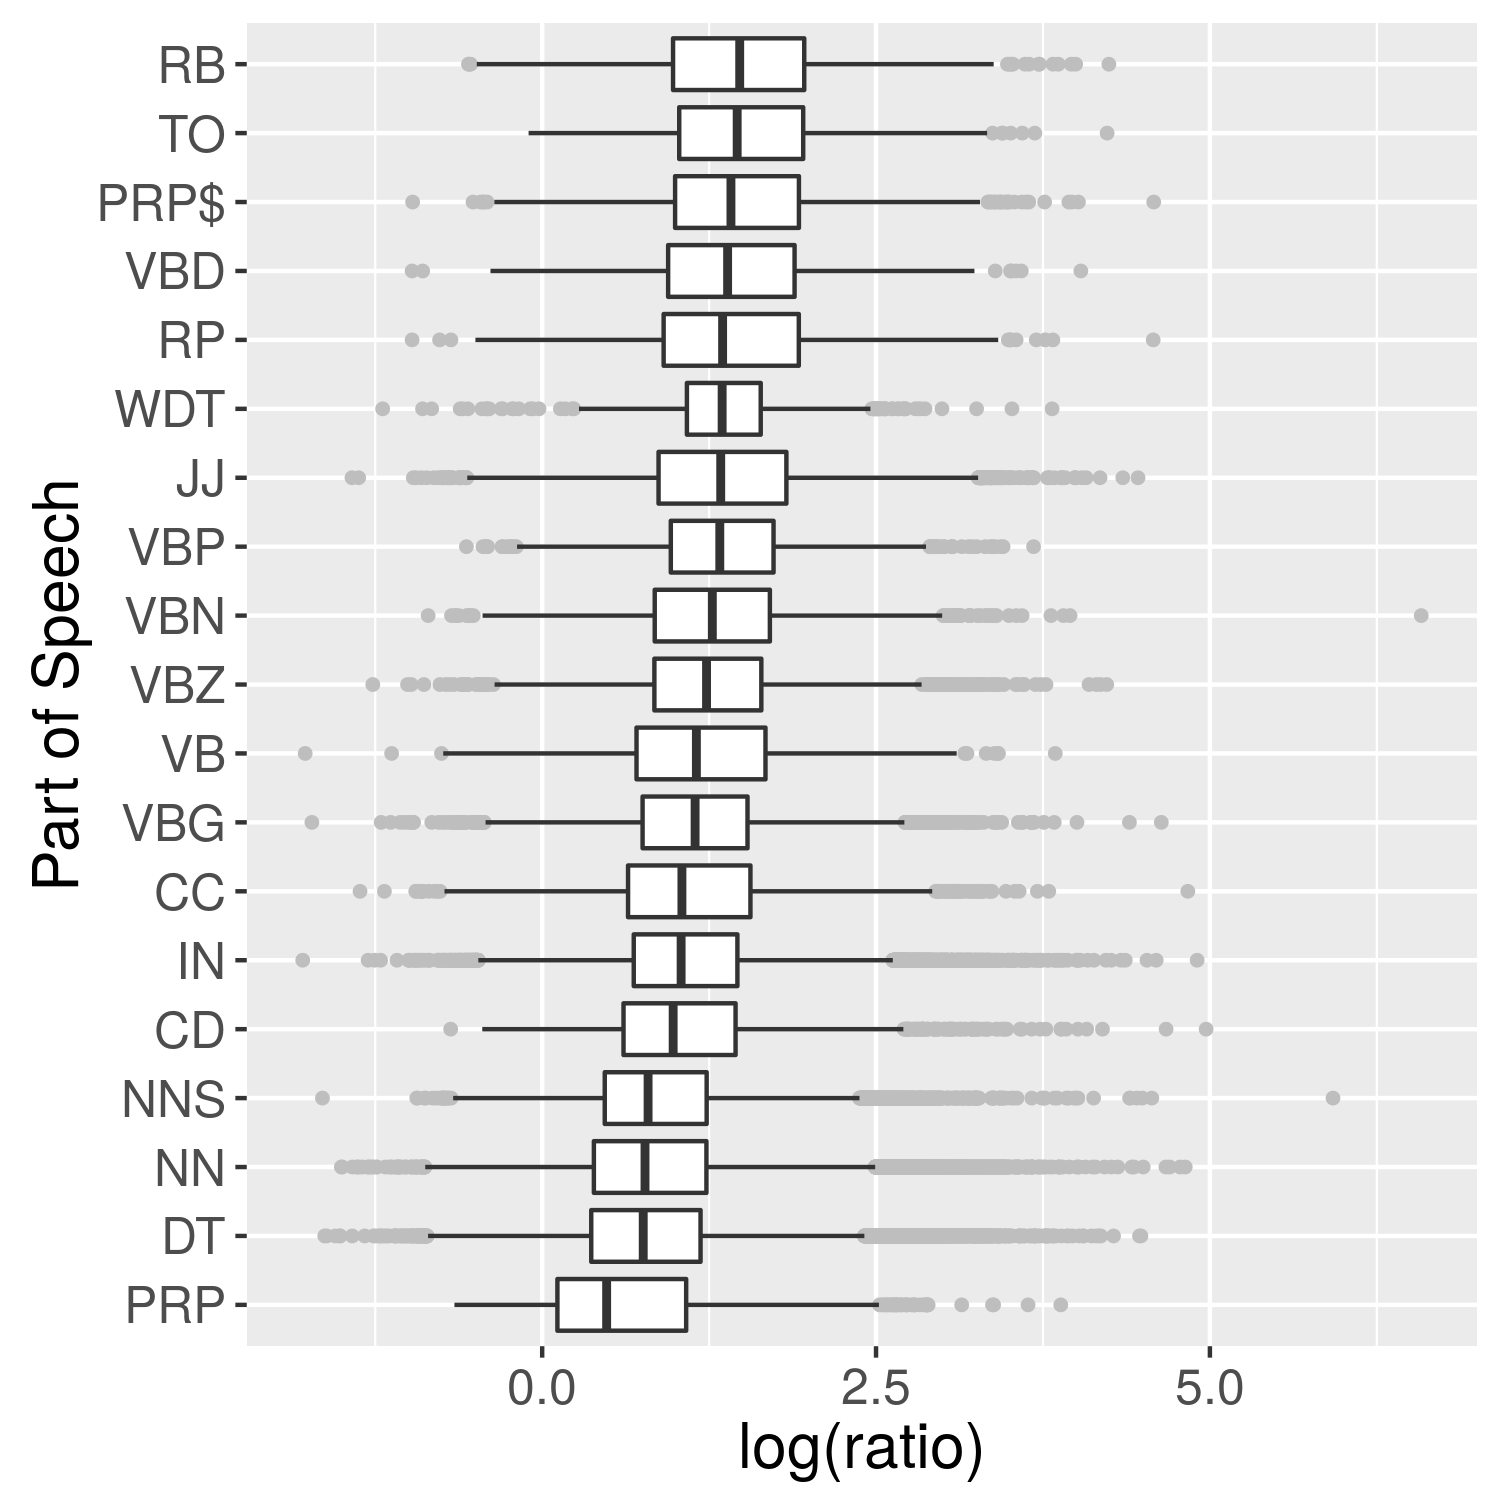
\includegraphics[scale=0.55]{imaginet-omission-quotient-pos-boxplot.png} &
  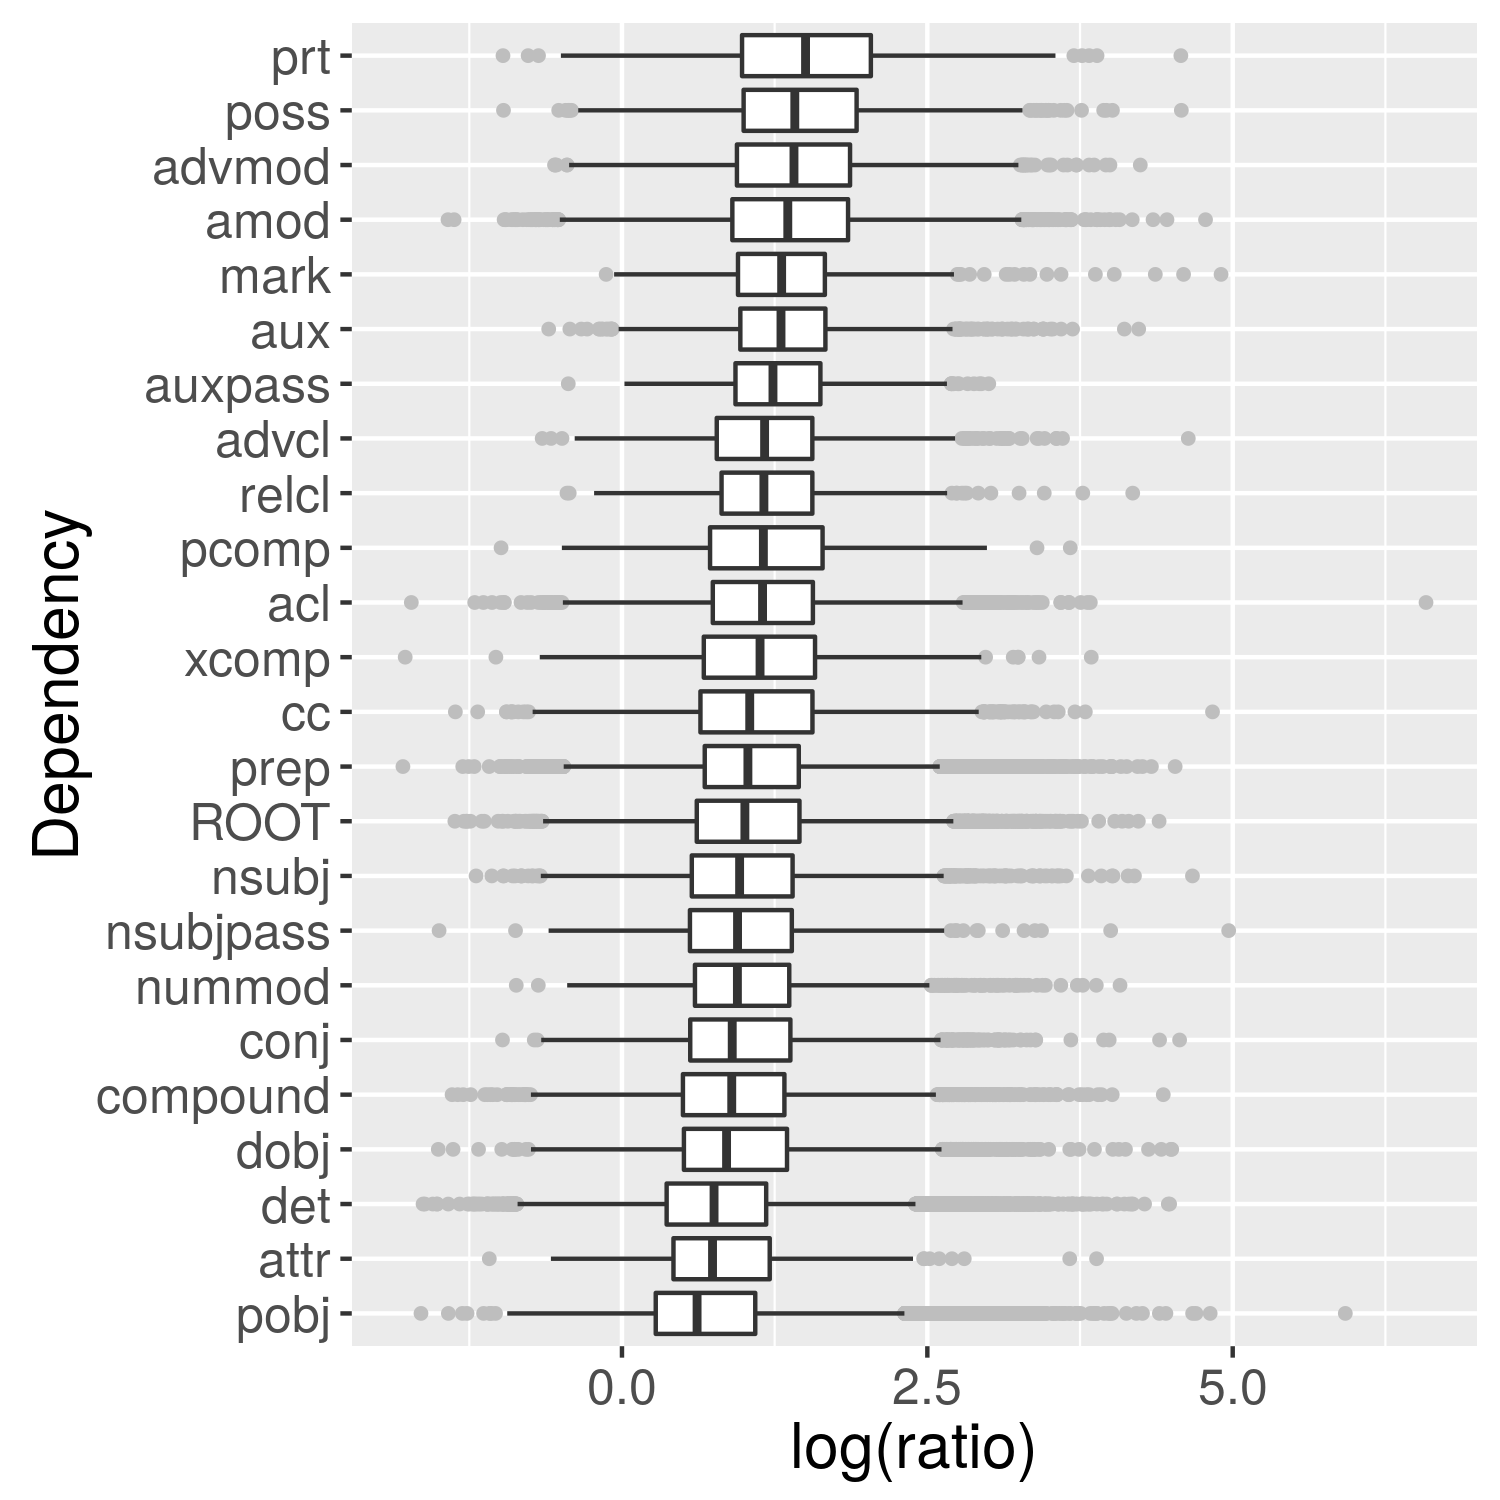
\includegraphics[scale=0.55]{imaginet-omission-quotient-dep-boxplot.png} \\  
  \end{tabular}
  \caption{Distributions of log ratios of omission scores of {\sc LM} to {\sc Textual} per
    POS (left) and dependency labels (right). Only labels which occur at least 500 times are included.}
\label{fig:omission-imaginet-ratio}
\end{figure*}


The $\mathrm{omission}$ scores can be used not only to
estimate the importance of individual words, but also of syntactic
categories. We estimate the salience of each syntactic category by
accumulating the omission scores for all words in that category. We
tag every word in a sentence with the part-of-speech (POS) category
and the dependency relation (deprel) label of its incoming arc. For
example, for the sentence \emph{the black dog}, we get ({\it
  the},~DT,~det), 
({\it black},~JJ,~amod), ({\it dog},~NN,~root). 
Both POS tagging and dependency parsing are performed jointly
using the TurboParser dependency parser \cite{martins2013turning}.\footnote{Available at
  \url{https://github.com/andre-martins/TurboParser}{github.com/andre-martins/TurboParser}.} The POS tags used are the Penn Treebank tags and the dependencies are 
the Stanford basic dependencies.


Figure~\ref{fig:omission-imaginet} shows the distribution of omission
scores per POS and deprel label for the two pathways of {\sc Imaginet}. 
The general trend is that for the {\sc Visual} pathway, the omission scores are
high for a small subset of labels - corresponding mostly to nouns, less so for
adjectives and even less for verbs - and low for the rest (mostly function words and
various types of verbs). For {\sc Textual} the differences are \label{edit:textualomission}
smaller, and the pathway seems to be sensitive to the omission of most
types of words.  

Figure~\ref{fig:omission-imaginet-ratio} compares the
two pathways directly using the log of the ratio of the {\sc Visual}
to {\sc Textual} omission scores, and plots the distribution of this
ratio for different POS and deprel labels.  Log ratios above zero
indicate stronger association with the {\sc Visual} pathway and below
zero with the {\sc Textual} pathway. We see that in relative terms,
{\sc Visual} is more sensitive to nouns (NNP, NNS, NN), numerals (CD)
and adjectives (JJ), and {\sc Textual} to the prepositions (TO, IN),
some types of verbs (VBZ, VBP), determiners (DET, WDT) and
particles (RP). This picture is complemented by the analysis of the
relative importance of dependency relations: {\sc Visual} pays most
attention to the relations {\sc nsubjpass, nsubj, pobj, root, dobj,
  nn, conj, dep, amod} and {\sc num}, whereas {\sc Textual} is more
sensitive to {\sc det, mark, aux, auxpass, prt, prep, poss, cc} and
{\sc cop}. 

As expected, {\sc Visual} is more focused on grammatical
functions typically filled by semantically contentful words, while
{\sc Textual} distributes its attention more uniformly and 
attends relatively more to purely grammatical functions. 
It is worth noting, however, the relatively low omission scores for verbs in case \label{edit:generality}
of {\sc Visual}. One might expect that the task of image prediction from
descriptions requires general language understanding and so high omission
scores for all content words in general, however, the results
suggest that this setting is not optimal for learning useful representations of verbs,
which possibly leads to representations that are too task specific 
and not transferable across tasks. 


%The results on syntactic categories for {\sc Visual} are somewhat similar to 
%{\sc Sentiment} in that both models seem to learn to focus on one
%particular category (Nouns for {\sc Visual}, Adjectives for {\sc Sentiment}). 
%{\sc Visual} still incorporates adjectives, personal
%pronouns and verbs to the representations, but tends to ignore
%words of other categories. 


\subsection{Beyond Lexical Cues}
\label{sec:beyondlexical}

Models that utilize the sequential structure of natural-language 
have the capacity to interpret the same word-type differently depending on
the context. The omission score distributions in Section \ref{sec:omitimaginet} 
show that in the case of {\sc Imaginet} the 
pathways are differentially sensitive to content vs.\ function
words. This may be either just due to purely lexical features or the model 
may actually learn to pay more attention to the same word type in appropriate
contexts. This section investigates to what extent {\sc Visual} and {\sc Textual}
discriminate between occurrences of a given word in different positions and 
grammatical functions. The analysis we described here takes \label{edit:beyonlexicalgeneral}
the omission scores as input data, therefore it can be potentially applied 
to any architecture for which the omission scores can be computed. However,
the presented analysis and results regarding word positions can only be meaningful
for Recurrent Neural Networks as they compute their representations sequentially and are not
limited by fixed window sizes.\footnote{CNNs with multi-word filters
and tree-structured recursive neural networks do not incrementaly build representations
of sentences in a left-to-right or right-to-left fashion. 
Bi-directional RNNs, however, are affected by word-order and can potentially
learn to handle the same word in different positions differently. \label{edit:foot}}

We fit four L2-penalized linear regression models which predict the omission 
scores per token with the following predictor variables: 


\begin{enumerate}
	\item {\sc LR word}: word type
	\item {\sc LR +dep}: word type, dependency label and their interaction 
	\item {\sc LR +pos}: word type, position (binned as {\sc first, second, third, middle,
	antepenult, penult, last}) and their interaction
	\item {\sc LR full}: word type, dependency label, position, word:dependency interaction, 
	word:position interaction
\end{enumerate}

\noindent We split the 5-thousand-image portion of MSCOCO validation data into two parts, fit the 
models (regularized via L2 penalty) on the first part, and compute the 
proportion of variance explained on the second part. 
For comparison we also train a version of {\sc Imaginet},
where the GRU in the {\sc Visual} pathway is replaced by a simple vector-summation operation
over word-embeddings and thus does not have access to sequential cues. We refer to this
model as {\sc Sum}. 

\begin{table}
  \centering
  \caption{Proportion of variance in omission scores explained by
    linear regression.}
    \begin{tabular}{l|rrrr}
               & word   & +pos  & +dep  & full \\\hline
     sum       & 0.654  & 0.661 & 0.670 & 0.670 \\
     LM        & 0.358  & 0.586 & 0.415 & 0.601 \\
     textual   & 0.364  & 0.703 & 0.451 & 0.715 \\
     visual    & 0.490  & 0.506 & 0.515 & 0.523 \\
    \end{tabular}
    \label{tab:lr-r2}
\end{table}

Table~\ref{tab:lr-r2} shows the proportion of variance $R^2$ in omission
scores explained by the linear regression with the different predictors.
Figure~\ref{fig:rsquared} offers a different view of the data, showing
the increase or decrease in $R^2$ for the models per pathway relative to {\sc LR
  +pos}.  The results reveal that adding additional information on
top of lexical features in case of {\sc Sum} does increase the
explained variance slightly, which is probably due to the unseen words
in the held out set. More interestingly, there is a sizeable
increase in $R^2$ between {\sc LR +pos} and {\sc LR full} in
case of {\sc Visual}, suggesting that 
the omission scores in case of {\sc Visual} depend on the words'
grammatical function in sentences, even after controling for word
identity and linear position.  

The raw $R^2$ scores show that for the {\sc Textual} and {\sc LM}
models the word-type predicts the omission-score to much smaller
degree compared to {\sc Visual}, and the increase in $R^2$ shows that
the position of the word adds considerable amount of information for
these language models: this is not surprising considering that the omission
scores are measured with respect to the final activation state. 
Less predictably, for the {\sc Visual} model,
dependency labels are more informative than linear position,
hinting at the importance of syntactic structure beyond linear order.

Overall, when regressing on word identities, word position and
dependency labels, the {\sc Visual} model's omission scores are the
hardest to predict of the four models suggesting that the model may be
encoding additional structural features not captured by these
predictors.

\begin{figure}
\centering
  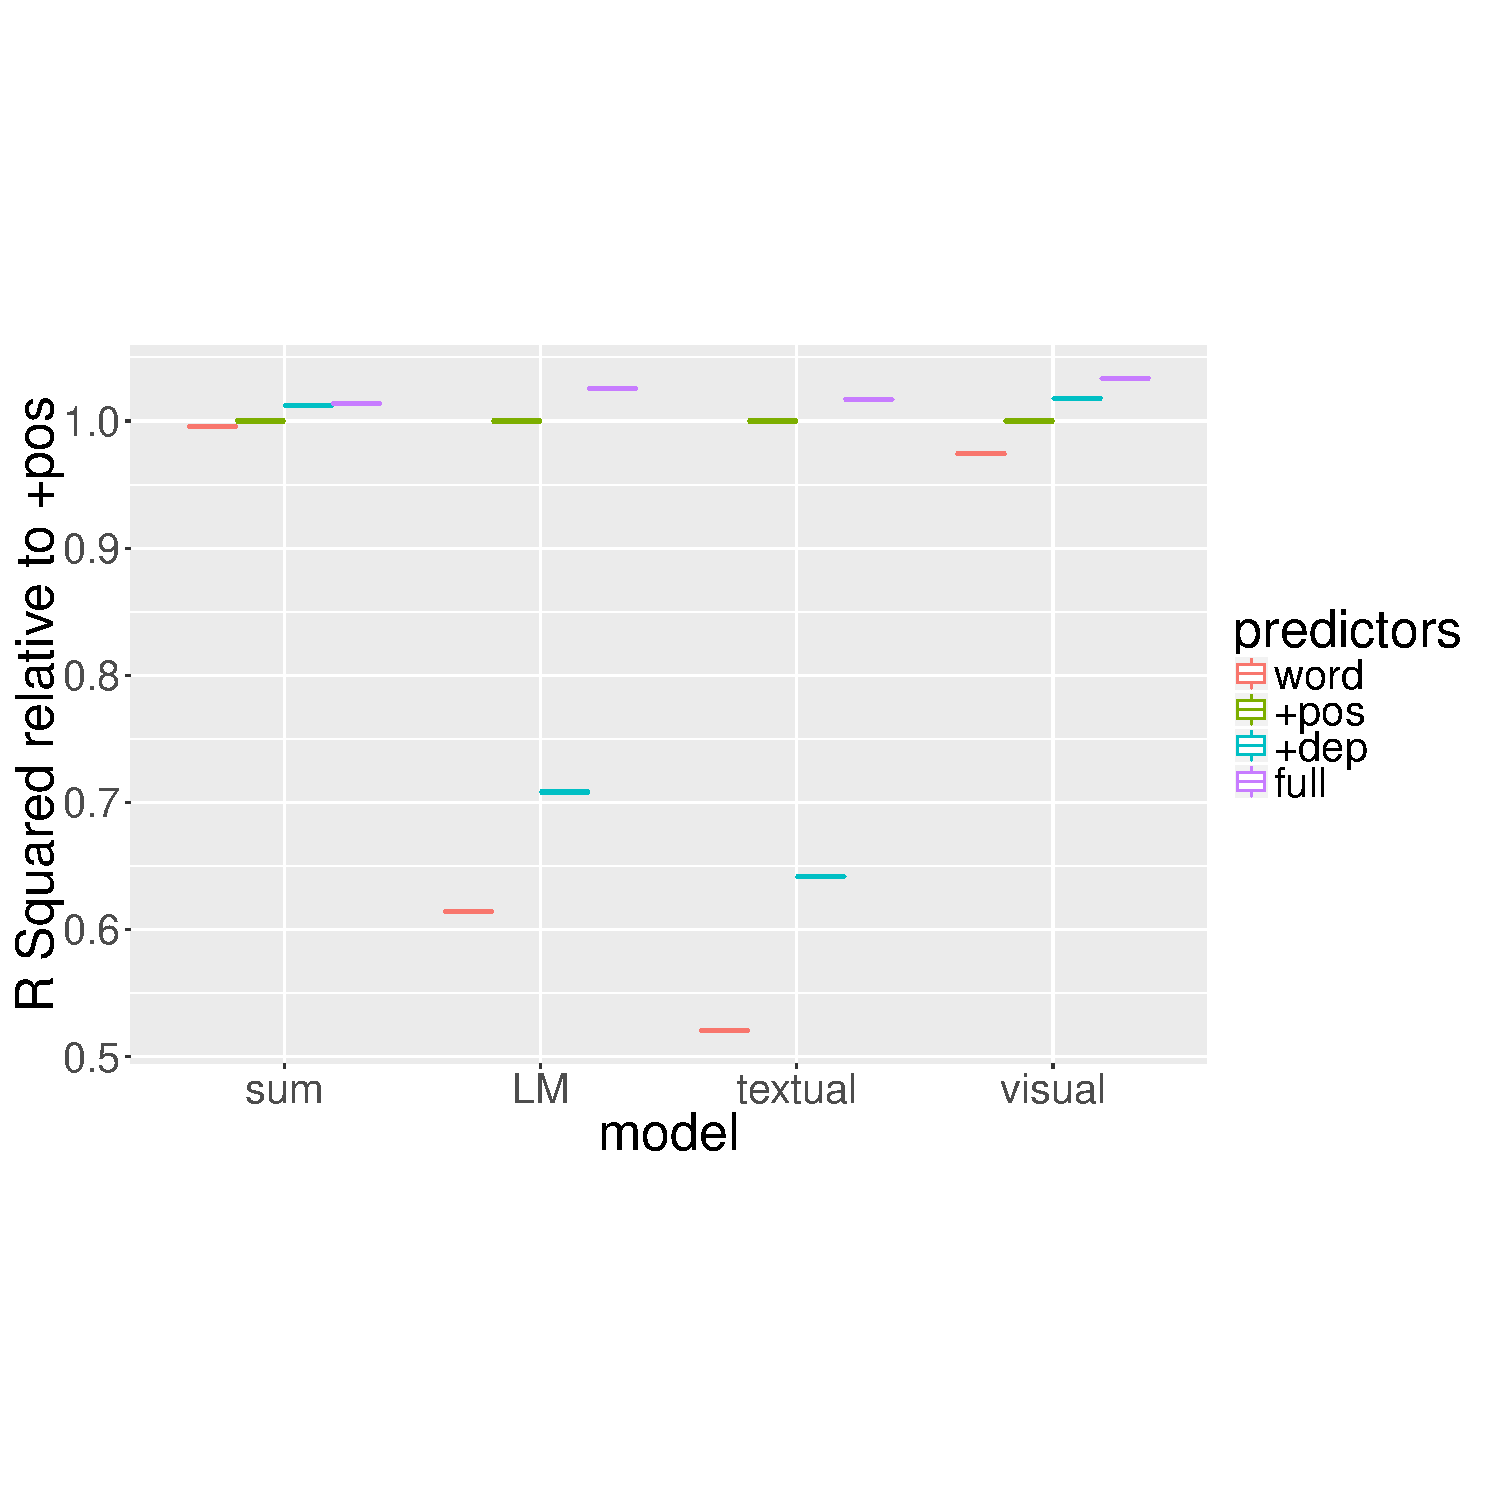
\includegraphics[scale=0.35]{position-new.pdf}
\caption{Proportion of variance in omission scores explained by the
  linear regression models
 for {\sc Sum}, {\sc Visual} and {\sc Textual} pathways, relative to
 regressing on word identity and position only. }
\label{fig:rsquared}
\end{figure}


\subsubsection{Sensitivity to grammatical function}
\label{sec:gramfunc}

%\begin{figure}[t]
%  \centering
%  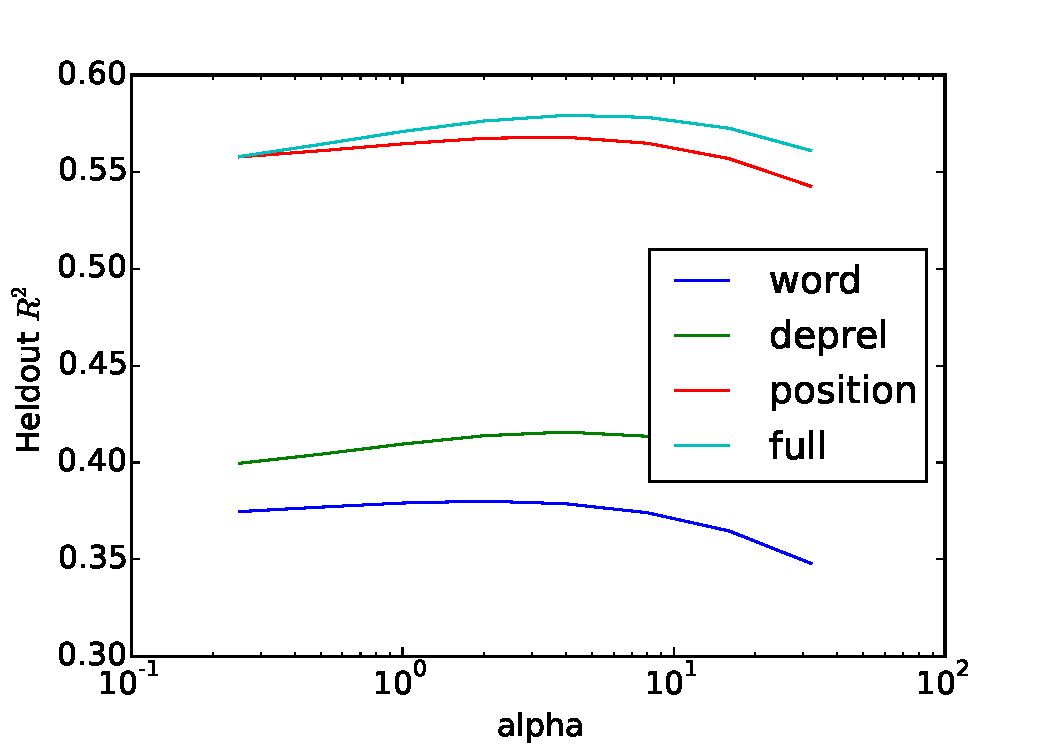
\includegraphics[scale=0.4]{omission-stat/scores-vs-alpha.pdf}
%  \caption{Proportion of variance in omission scores explained by {\sc Model 1} vs {\sc Model 2} as a function of regularization parameter $\alpha$.}
%  \label{fig:scores-vs-alpha}
%\end{figure}




\begin{figure}[t]
  \centering
  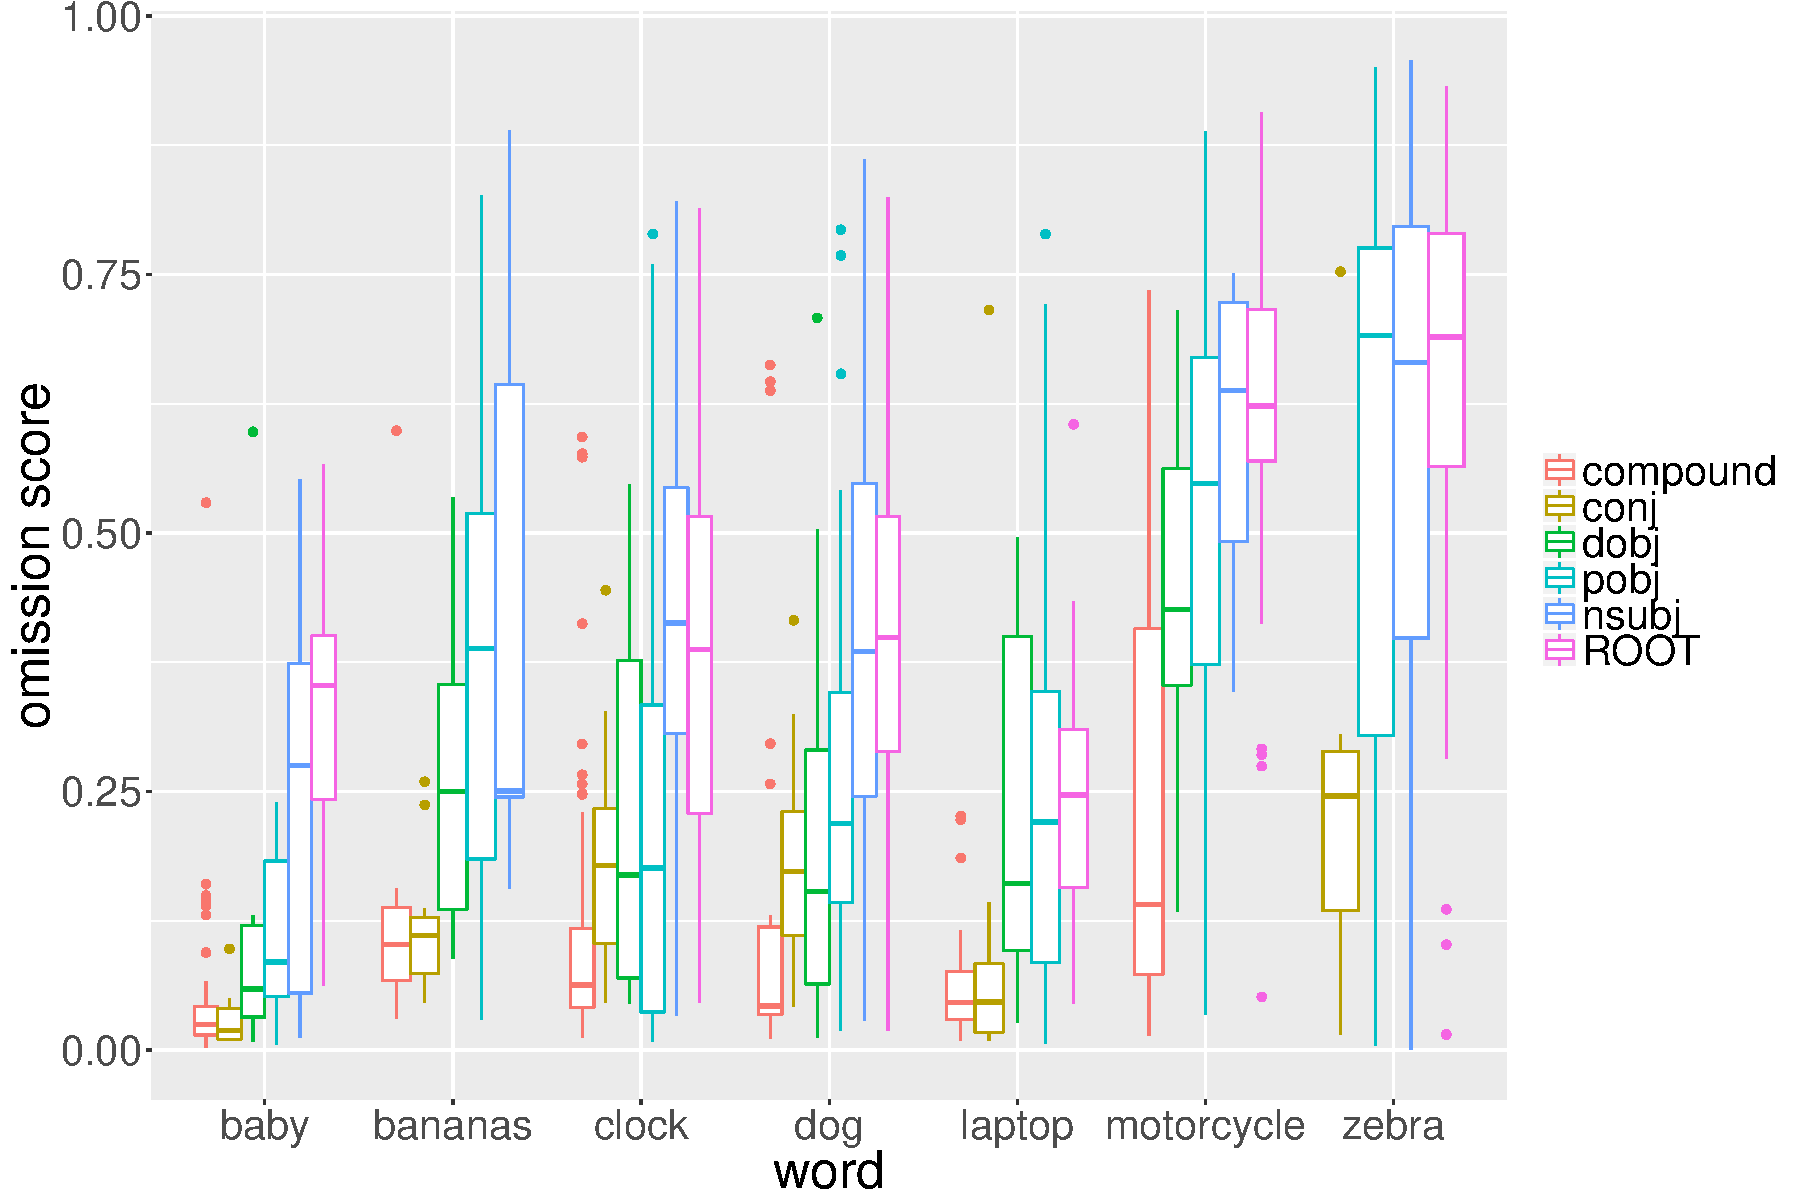
\includegraphics[scale=0.35]{top_words.pdf}
  \caption{Distribution of omission scores per deprel label for the selected word types.}
  \label{fig:top_words}
\end{figure}
%\todo{At some point redo this with words ranked by ratio between the errors not the difference}

In order to find out some of the specific syntactic configurations leading to
increase in $R^2$ between {\sc LR word} and {\sc LR dep} predictors
in case of {\sc Visual}, we next considered all word types with
occurrence counts of at least 100 and ranked them according to how much
better, on average, {\sc LR +dep} predicted their omission scores 
compared to {\sc LM word}. 

Figure~\ref{fig:top_words} shows the per-dependency 
omission-score distributions for the five top ranked words plus the word {\it  water}. 
There are clear and large differences in how these words
impact the network's representation depending on what grammatical
function they fulfill. They all have large omission scores when they
occur as {\sc nsubj} (nominal subject) or {\sc root}, likely due to the fact that these
grammatical functions typically have a large contribution to the
complete meaning of a sentence.  Conversely, all have small omission 
scores when appearing as {\sc conj} (conjunct): this is probably because in this position
they share their contribution with the first, often more important,
member of the conjunction (e.g. {\it A cow and its baby eating
  grass}). 
  
The pattern for {\sc nn} (nominal modifier) is a bit more complicated: for
four of the words shown (as well as for most other words not shown in
the figure), the score is very low in this grammatical function--presumably 
because most words contribute less to the sentence meaning when used  
as modifiers than as heads (e.g.\ {\it a clock tower}). However,
for the words {\it zebra} and {\it water}, omission scores are high
when they act as a nominal modifier {\sc nn}. This appears due to two reasons:
\begin{enumerate}
\item For {\it zebra}, there are frequent erroneous parses such as {\it
    zebra/{\sc nn} browsing/{\sc root}} instead of {\it zebra/{\sc nsubj} browsing/{\sc
    root}}. The network does not make this mistake, and treats these
    occurrences of {\it zebra} according to its importance as {\sc nsubj}.
\item {\it Water} as a modifier often changes the meaning of its head in
 a visually salient way: e.g.\ {\it water fall, water balloon, water scene, water skiing}, and
  thus the network learns that this particular word is important in the modifier position.
\end{enumerate}

\subsubsection{Sensitivity to information structure}
\label{subsec:information-struct}

\begin{figure}
\centering
 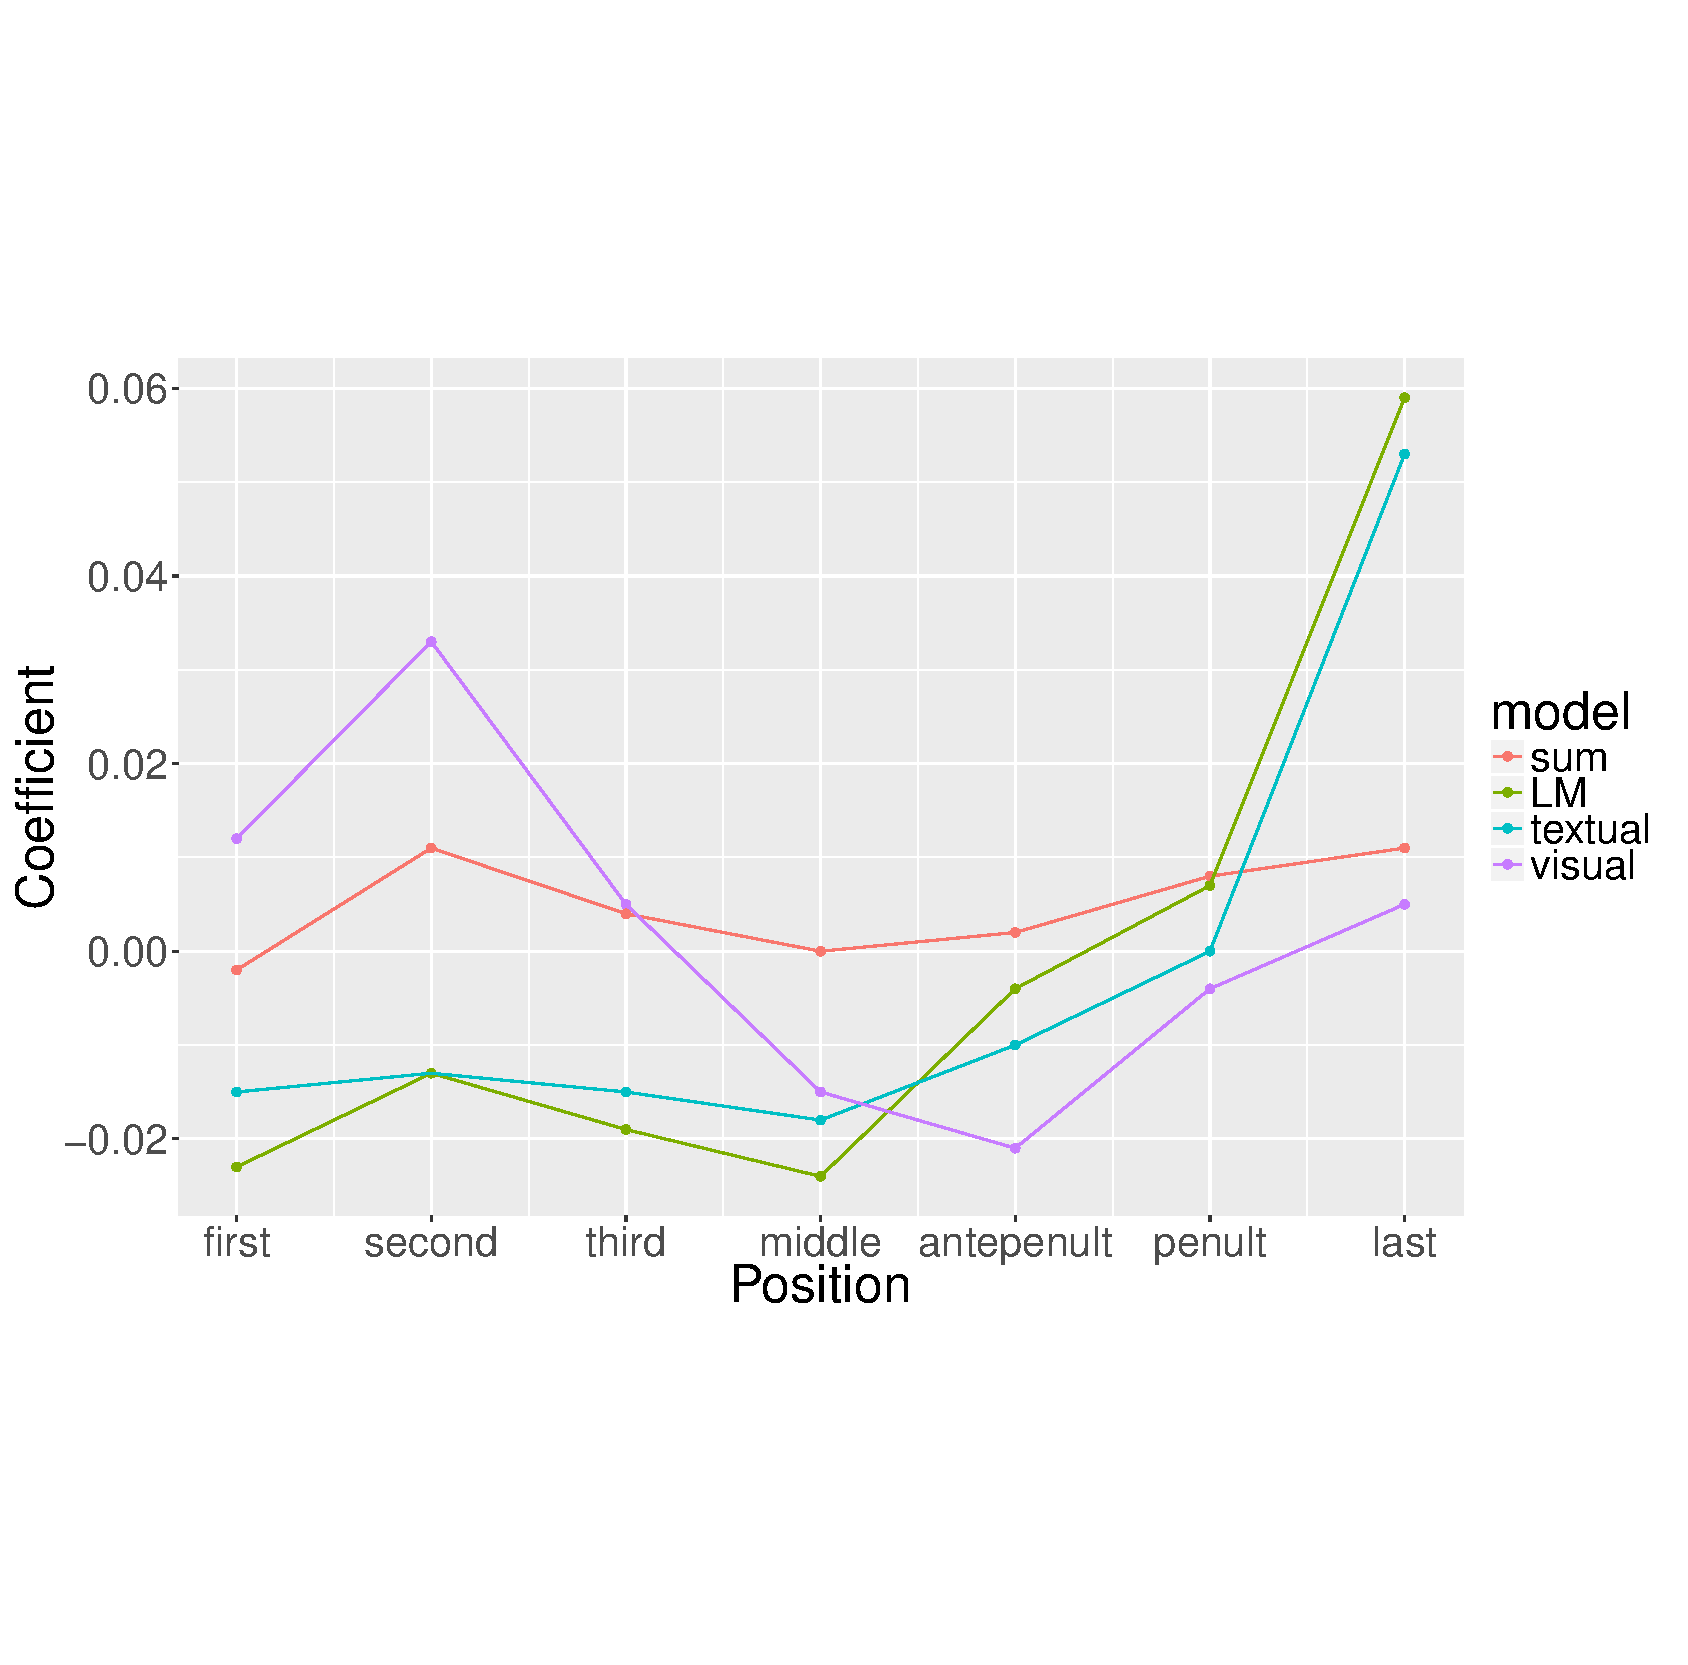
\includegraphics[scale=0.4]{position-coef.pdf}
 \caption{Coefficients on the y-axis of {\sc LM full} corresponding to the
position variables on the x-axis.}
 \label{fig:posrqs}
\end{figure}
 
As observed in Section \ref{sec:beyondlexical}, 
adding extra information about the position of words 
explains more of the variance in case of {\sc Visual} and especially {\sc Textual}.
Figure \ref{fig:posrqs} shows the coefficients corresponding to the
position variables in {\sc LM full}. Since the omission scores 
are measured at the end-of-sentence token, the expectation is that 
for {\sc Textual}, as a language model,  
the words appearing closer to the end of the sentence would have a
stronger effect on the omission scores. This seems to be confirmed by
the plot as the coefficients up until the \emph{penultimate} are all negative.


For the {\sc Visual} model it is less clear what to
expect: on the one hand due to their chain structure,  
RNNs are better at keeping track of
short-distance rather than long-distance dependencies and thus we can expect 
tokens in positions closer to the end of the sentence to be more important. 
On the other hand in English the information structure (or pragmatic structure) 
of a sentence is expressed via linear ordering: the {\sc topic} of a 
sentence appears sentence-initially, and the {\sc comment} follows. 
In the context of other text types such as dialog or multi-sentence \label{edit:topiccomment}
narrative structure, we would expect {\sc comment} to often be more
important than {\sc topic} as {\sc comment} will often 
contain new information in these cases. In our setting of image captions 
however, it is the {\sc topic} that typically contains the most important 
objects depicted in the image, e.g. {\it {\underline{two zebras}} are grazing in tall grass on a savannah.}
Thus, for the task of predicting features of the visual scene, it would 
be advantageous to detect the topic of the sentence and up-weight its
importance in the final meaning representation. Figure \ref{fig:posrqs}
appears to support this hypothesis and the network does 
learn to pay more attention to  words appearing
sentence-initially. This effect seems to be to some extent mixed with the recency
bias of RNNs as perhaps indicated by the relatively high coefficient of the {\it last}
position for {\sc Visual}. 


% The basic idea is to focus on
% words which occur in several grammatical functions, and see whether
% the network treats the different occurrences differently based on the
% dependency label. 

% The omission score results for {\sc Visual}
% suggest that the model pays relatively more attention to 
% categories {\sc nsubj, pobj, root} than to {\sc nn}. 
% Since the same word types can potentially
% assume these categories in different contexts which leads to the
% hypothesis that {\sc Visual} learned to recognize small syntactic 
% constructions. In the following experiment we consider word types 
% that appear with all four of the following dependency labels: 
% {\sc nsubj, pobj, root, nn}. Table \ref{tab:nnexample} demonstrates
% examples of the systematic pattern that in when tokens with deprel {\sc nn}
% have the lowest 

% A systematic pattern that provides evidence to support
% the hypothesis is that when nouns assume the role of noun complement
% {\sc nn}, their omission score is the lowest. This result is illustrated
% in 

% \iffalse
% \subsection{Distribution of omission scores}

% Determining feature importances from RNN hidden states for NLP tasks
% allows to uncover what kinds linguistic features models focus on.  We
% showed that omission scores allow for interesting qualitative
% comparison between RNN based models, but also provides insight into
% the nature of the combinations of data sets and tasks. The omission
% score results shows that to estimate the polarity of the sentence a
% model should primarily focus on adjectives. More interestingly the
% relative higher omission scores for Nouns for {\sc Visual} suggests
% that combination of the MS-COCO data set and the pre-trained VGG-CNN
% image-representation prediction as objective does not seem to promote
% the model to learn to pay attention to verbs. This analysis suggests
% that this particular setting does not allow the model to learn general
% representations for phrases/sentences as it promotes filtering out the
% information content of verbs.  Relative to {\sc Visual} the
% omission-score distribution of the {\sc Skip-gram} is much flatter
% providing an indication that the model does not throw away as much
% important linguistic information.  \todo{show some plot of the
%   distributions VISUAL vs. skip-gram} \fi
